\scanpage{94}
de $\pi_0$, $\pi'_0=\operatorname{Im}(\pi_1(\widetilde{\unsure{\mathcal{T}|\mathcal{C}}},x'_0)\unsure{-|\longrightarrow}\pi_1(\unsure{\mathcal{T}|\mathcal{C}},x_0))$, de sorte que
\[
\unsure{(47)}\qquad E_0\simeq\pi_0/\pi'_0;
\]
\deleted{$\unsure{\widetilde{\mathcal{T}}}$}
la condition d'existence de $\widetilde{\Theta}_0$ revient à dire
\[
\Theta(\pi'_0)\text{ conjugué à }\pi'_0\text{ dans }\pi_0
\]
\margin{en effet, il faudra que $\Theta(\pi'_0)$ soit $\operatorname{Im}(\pi_1(\widetilde{\unsure{\mathcal{T}|\mathcal{C}}},x'_1)\to\pi_1(\unsure{\mathcal{T}|\mathcal{C}},x_0))$, où $x'_1=\widetilde{\Theta}(x'_0)$, ou si $x'_1=g(x'_0)$, avec $g\in\pi_0$, l'Im en question est $\operatorname{int}(g)(\pi'_0)$.}
et les choix possibles pour remonter $\Theta$ en $\widetilde{\Theta}_0$, donc pour remonter $\Theta$ en $\widetilde{\Theta}$, correspondent aux éléments \inserted{$\unsure{x'_1}$} de $E_0$ \deleted{tels que} \inserted{de la} forme $g(x'_0)$ avec $g\in\pi_0$ satisfaisant
\[
(48)\qquad \operatorname{int}g(\pi'_0)=\Theta(\pi'_0)
\]
i.e. tels que
\[
g\in\operatorname{Transp}_{\pi_0}(\pi'_0,\Theta(\pi'_0))
\]
\margin{Cette condition ne dépend que de l'endom. \uline{ext.} défini par $\Theta$ sur $\pi'_0$ --- mais la façon de remonter $\Theta$ en $\widetilde{\Theta}$, $\unsure{=}$ \unsure{comme endom. ext., en dépend}, \unsure{aux de l'} \uline{\unsure{pas}} \unsure{un} endom. ord. \unsure{défini} par $\Theta$.}
\margin{\deleted{\unsure{Si} $\unsure{\widetilde{\mathcal{T}}}$ \unsure{correspond} \illegible{3} \unsure{on a} $\unsure{\Theta'_0}$ \illegible{3} $\unsure{\Theta}$ \illegible{2} $\unsure{\widetilde{\Theta}}$ \unsure{tel que} $\unsure{\exists\gamma\in\pi_0}$ \unsure{avec} $(48\,\mathrm{bis}):\ \unsure{\Theta}(\unsure{\pi'_0|x'_0})=\unsure{\gamma}(\unsure{\pi'_0|x'_0})$ \unsure{dans} $\pi'_0$.}}
donc les $\Theta$ possibles correspondent aux éléments de
\[
(49)\qquad \operatorname{Transp}_{\pi_0}(\pi'_0,\Theta(\pi'_0))/\pi'_0
\]
\margin{espace homogène à droite ($\pi'_0$ opère à droite sur le transporteur, via $g\longmapsto g\alpha$ pour $\alpha\in\pi_0$.}
\margin{Bien sûr, les façons de remonter $\Theta$: $\Theta'$ de $\mathcal{T}'\subset\widetilde{\mathcal{T}}$ correspondent aux $\widetilde{\Theta}$ qui rendent bien ainsi $\mathcal{T}'\subset\widetilde{\mathcal{T}}$ invariant.}

Ainsi, on voit que dans le cas \deleted{$\unsure{\mathcal{T}}$}
\[
\mathcal{T}=\widehat{\Pi}_1(X_{\unsure{\overline{k}}},I),\qquad I\subset X_{\unsure{k}}
\]
quand $\mathcal{T}'$ \deleted{\unsure{en premier}} est de la forme $\widehat{\Pi}_1(X'_{\unsure{\overline{k}}},I')$, où $X'$ est un rev. étale (fini) de $X$, \inserted{avec $I'\to I$}, que la condition qu'un $\Theta$ \inserted{de $\mathcal{T}$} se remonte en un \unsure{autom.} de $\mathcal{T}'$ est une condition algébrique des plus
\mspage{93}

\scanpage{95}
\mspage{15}
\deleted{plus} simples, qui pour $I'=p^{-1}(I)$ ne dépend pas du choix de $I'$ i.e. de $I$. Si on veut que l'action remontée $\Theta'$ soit l'identité sur $I'$, \unsure{on écrit}, et la condition supplémentaire que $\widetilde{\Theta}$ doit bien opérer \uline{trivialement} sur $I'$.

Revenons à l'action de $\Gamma$ \inserted{$=\operatorname{Gal}\overline{K}/K$} sur un $\mathcal{T}=\deleted{\unsure{\Pi_1}}\widehat{\Pi}_1(X,I)$ avec $I\subset X_K$, on trouve donc une condition nécessaire pour qu'un \unsure{autom.} $\Theta$ de $\mathcal{T}$ \inserted{trivial sur les objets} provienne d'un $u\in\Gamma$:

\margin{Ces deux conditions ne dépendent en fait que de l'opération de \deleted{$\unsure{\Theta}$} $\Theta$ sur le groupe fondamental en \uuline{un} point $x_0\in I$.}
a) Pour tout rev. \inserted{étale} fini $X'$ de $X$, \inserted{(défini sur $K$)} \deleted{\unsure{il considère l'action de}} \inserted{\unsure{il y a} une action $\widetilde{\Theta}$} de $\Theta$ sur $\widehat{\Pi}_1(X',I')$, où $I'=X'|I$, qui remonte $\Theta$, et qui est l'identité sur $I'\cap X'_K$.

b) De plus, pour $\forall$ hom. (défini sur $K$)
\[
X'\xrightarrow{f}Y
\]
et tout $x'\in I'\cap X'_K$, le noyau de
\[
(*)\qquad\widehat{\pi}_1(X',x')\longrightarrow\widehat{\pi}_1(\unsure{X|Y},f(x')),
\]
est stable sous $\unsure{\widetilde{\Theta}^{\prime}|\widetilde{\Theta}}$ \inserted{(pour $\widetilde{\Theta}$ convenable!)} --- plus généralement, sans supposer $x'\in X'_K$, mais choisissant $\nu\in\unsure{\mathbb{N}|\mathbf{N}}^{+}$ tel que $\Theta^\nu x'=x'$, il faut que \deleted{$\unsure{\Theta}$} le noyau de $(*)$ soit stable par $\Theta^\nu$.

\margin{\uline{NB} Ces conditions \unsure{deviennent informulables}, \unsure{tant qu'on se borne à ne parler que} des actions \uline{extérieures} de $\Gamma$!}
Ce sont là des conditions draconiennes. Je pense que ce n'est pas trop m'avancer,
\mspage{94}

\scanpage{96}
en conjecturant que ces conditions \inserted{nécessaires} sont suffisamment draconiennes \deleted{pour} (même sans entrer ds la considération des $\Theta'$) pour assurer que $\Theta$ provient bien d'un $u\in\Gamma$, \deleted{\unsure{pour}} lorsque $X$ est (disons) une \uline{courbe algébrique anabélienne}, avec extension de type fini de $\mathbf{Q}$.
\margin{Je ne vois pas très bien si la condition a) \inserted{\unsure{fixe $x_0$ de point générique}}, sans b), devrait suffire pour assurer que $\Theta$ vient de $\Gamma$. Et puis, \unsure{$K$ est de t.f.} \unsure{sur tous ces objets, dans le groupe profini} \unsure{de $\Gamma$}.}
\margin{Il n'est pas évident que l'hypothèse anabélienne soit requise --- à examiner! (\unsure{N'est-ce pas?}). Pour $\mathbf{G}_m$, ou une courbe elliptique, la variation: $X/K$ \unsure{me semble également} \unsure{inessentielle}. \uline{En fait, c'est faux pour $\mathbf{G}_m$}.}
Bien sûr, la question de l'unicité de $u$ n'est pas \unsure{impliquée|indiquée} ici --- quand $K$ est une extension algébrique de $\mathbf{Q}$, on s'attend à l'\uline{unicité} de $u$. Quand $K$ est de degré de transcendance $>0$, alors pour pouvoir s'attendre à l'unicité de $u$, il faut au moins supposer que le corps modulaire de $X$ a ce degré de transcendance, i.e. que $K$ est une extension \uline{finie} de ce corps modulaire. Je ne serais pas étonné qu'on ait unicité dans ce cas.
\margin{Ça doit \unsure{alors se ramener au premier des cas, via l'application de} \unsure{Белый|Belyi}. \unsure{Pour l'unicité, bien sûr, la condition} \unsure{a)} \unsure{absolument analogue}\unsure{...!}}

Je reviens sur la question de la relevabilité d'un \deleted{$\unsure{\Theta}$} endomorphisme $\Theta$ d'un groupoïde connexe $\mathcal{T}$ à un revêtement $\widetilde{\mathcal{T}}$, quand $\Theta$ fixe un sommet
\mspage{95}

\scanpage{97}
\mspage{16}
$x_0$ de $\mathcal{T}$, mais sans supposer maintenant $\widetilde{\mathcal{T}}$ connexe. (En pensant au cas où $\widetilde{\mathcal{T}}$ proviendrait d'une situation géométrique $X'\unsure{-|\to}X$, avec $X$ connexe, \deleted{\unsure{et un revêtement}} mais $X'$ seulement $K$-connexe i.e. connexe en tant que schéma sur $K$ --- ce qui signifie qu'il \deleted{\unsure{se}} se décrit en termes galoisiens par $E_0=X'_{x_0}$, sur lequel le produit $\unsure{\frac12|s.}$ direct $\Gamma.\pi_0$ ($\pi_0=\pi_1(X,x_0)=\pi_1(\mathcal{T},x_0)$) opère transitivement, mais sans que l'opération de $\pi_0$ soit forcément transitive.) Associons à $\forall\ x'\in E_0$ son stabilisateur dans $\pi_0$, on trouve une application
\[
(50)\qquad
\diagram{\begin{tikzcd}[ampersand replacement=\&,column sep=large,row sep=small]
E_0 \arrow[r] \& \text{Ens des ss-groupes de }\pi_0 \\
x' \arrow[r,mapsto] \& \text{stabilisateur }\pi_{\unsure{x'|0x'}}
\end{tikzcd}}
\]
qui commute aux actions de $\pi_0$ (op. sur le $2^e$ ens par autom. intérieurs), d'où par passage aux quotients
\[
(51)\qquad
\diagram{\begin{tikzcd}[ampersand replacement=\&,column sep=large]
E_0/\pi_0\overset{\mathrm{def}}=\unsure{\{\pi_0\}|\pi_0}(E_0) \arrow[r,"\overline{\Sigma}:"] \& \operatorname{Ssgr}(\pi)/\pi
\end{tikzcd}}
\]
\inserted{c'est le $\pi_0$ dans le topos des $\pi$-ens.}
D'autre part, $\Theta$ opère sur le $2^{\text{ième}}$ mb de (51) par transport de structure, via \unsure{l'autom.} donné de $\pi$, et \unsure{là} une condition nécessai-
\mspage{96}

\scanpage{98}
évidente pour que $\Theta$ se relève en un $\widetilde{\Theta}$, c'est que l'image de l'application (51) soit \uline{stable} sous l'action de $\Theta$; en fait, l'action $\widetilde{\Theta}$ présomptive, restreinte à $E_0$, doit donner la compatibilité. \deleted{\unsure{Rien qu'en} \illegible{3} \unsure{Inversement}} \inserted{On voit donc qu'en deux pts de $\overline{\Sigma}$ conjugués sous $\Theta$, le degré de $\unsure{(52)|\overline{\Sigma}}$ (cardinal de la fibre) doit} \deleted{de stabilité} \deleted{\unsure{telle}} \unsure{qui par raison d'images signifie} justement qu'il existe une \deleted{$\unsure{\widetilde{\Theta}}$} \inserted{bijection}
\margin{\unsure{On lie} les deux conditions.}
\[
(52)\qquad \pi_0(\widetilde{\Theta}_0):\pi_0(E_0)\overset{\sim}{\longrightarrow}\pi_0(E_0)
\]
\deleted{telle que} qui soit compatible avec l'action de $\Theta$ sur le deuxième mb de (51). Ceci dit, pour \unsure{toute telle} relèvement, il existe bel \inserted{\unsure{p.e.}} et bien un $\widetilde{\Theta}$ qui l'induise, lequel $\widetilde{\Theta}$ est \inserted{$\widetilde{\Theta}_0:E_0\overset{\sim}{\to}E_0$ est compatible avec l'action de $\pi$ et l'action de $\Theta$ sur $\pi$ (cf (46))} \inserted{bien connu quand on} connaît ses valeurs $\widetilde{\Theta}(x_i)$ \deleted{\unsure{pour}} pour \uline{un} $x_i\in E_0$ dans chaque composante connexe de $E_0$ \ldots

Parmi les conditions nécessaires \inserted{importantes} pour un automorphisme $\Theta$ \unsure{d'un} $\widehat{\Pi}_1(X,I)$, $I\subset X_K$, pour provenir de $\Gamma$, j'ai oublié apparemment la plus importante de toutes, avec laquelle je travaille \deleted{\unsure{pourtant}} constamment --- à tel point que cela finit par sembler aller de soi!
\mspage{97}

\scanpage{99}
\mspage{17}
C'est la condition de compatibilité avec la ``structure à lacets'' --- dans le cas où $X$ est une courbe algébrique, disons (sinon, on sait bien qu'il faut introduire, dans le cas général, une ``structure à l'infini'' des groupoïdes fondamentaux \ldots). \margin{$\Vert$} Cette compatibilité \inserted{justement} s'exprime de façon particulièrement naturelle et élégante dans le contexte des groupoïdes, \unsure{$\{$} comme une condition de la nature d'une compatibilité à des morphismes de schémas (cf (39)) --- mais on \unsure{pourrait|prendrait} ici non des schémas de t.f. mais des schémas locaux épointés ou ``modèles'' épointés --- je vais revenir sur ce point de vue plus bas.

\uline{Remarque.} Revenant aux conditions a) b), il est clair d'emblée qu'elles sont indéchiffrables \inserted{(i.e. inexprimables)} en termes $\pm$ directs, comme des conditions portant directement sur les ``paramètres'' du type $g_e(u)$ (des paramètres \deleted{\unsure{comme}} \inserted{tels que} ceux désignés par $\alpha,\beta,\xi,\eta$ dans mon étude des autom. à lacets de $\pi_3$ \ldots) qui ``représentent'' un $u\in\Gamma$ (ici $\Gamma=\operatorname{Gal}\overline{\mathbf{Q}}/\mathbf{Q}$). \deleted{Pourtant} C'est pour cette raison que \unsure{le|la}
\mspage{98}

\scanpage{100}
conjecture énoncée plus haut (que ces conditions, plus la condition des lacets, \inserted{si on veut} sont suffisantes) n'est pas bien intéressante, de nature trop platonique. Mais \unsure{il|je} \deleted{\unsure{paraît}} \inserted{me} semble que via l'étude des multiplicités \unsure{MD|DM} $M_{g,\nu}$ et des groupes de Teichmüller, je suis en train de me rapprocher du point où une conjecture intéressante et plausible, en termes de propriétés internes des groupes profinis tels que $\widehat{\pi}_{0,3}$, finira par apparaître (en commençant par des conditions liées aux $M_{0,4},M_{0,\unsure{5|3}}\ldots$).
\margin{En un sens elles ont les \unsure{défauts}, \unsure{avec les bonnes} --- puisque je \unsure{donne explicitement} \unsure{des} conditions de nature \unsure{topologiques|géométrique}, qui ne \unsure{parlent} que des \uline{\unsure{orientations|revêtements}} (\unsure{finis}) \unsure{un connexe|d'un connexe}, \unsure{du} groupoïde fondamental $\widehat{\Pi}_1(X_K)$ \unsure{pour les} \unsure{groupes fondamentaux}. \inserted{\unsure{sur les sous-groupes profinis de} $\unsure{\widehat{\pi}_1}$} \deleted{\unsure{pour les}}}

Je passe en revue encore une fois, sous forme complétée, les conditions pour un automorphisme \inserted{$\Theta$} d'un groupoïde $\widehat{\Pi}_1(X,I)$, $I\subset X_{\overline{K}}$, \inserted{$I\cap\unsure{X_K|X_{\overline{K}}}\ne\varnothing$}, (je pense surtout, pour le moment, au cas $X=U_{0,3}$) provienne d'un $u\in\Gamma=\operatorname{Gal}\overline{K}/K$:

1) Condition des lacets (pour mémoire --- c'est sûrement la plus importante de toutes, de très loin!)

2) Condition de \unsure{Stabilité|stabilité} pour revêtements étales \deleted{de} $X'$ de $X$ (définis sur $K$, bien sûr)\unsure{;|.}
\mspage{99}

\scanpage{101}
\mspage{18}
\margin{De plus, il y a lieu d'exiger \unsure{1°} que $\Theta$ soit trivial sur $\unsure{I'\cap X'_K}$, et qu'une puissance $\Theta^{\unsure{\nu K}}$ de $\Theta$ $(\nu\geq1)$ soit \unsure{triviale} sur $I$. Car $X'_K\ne\varnothing$ implique alors que $X'$ est $\unsure{+}$, $\unsure{=}$ connexe. \deleted{De plus}}

de $\Theta$ se relève en une action de $\Theta$ sur $\widehat{\Pi}_1(X',I')$, où $I'=X'\vert I$.
\deleted{$\unsure{\exists a'\in}$} $I'\cap X'_K\ne\varnothing$, $X'$ \unsure{étant|ét.} connexe (il suffit que $\Gamma$ soit transitif sur $\pi_0(X')$ i.e. que $X'$ soit ``$K$-connexe'' i.e. connexe en tant que schéma sur $K$) alors l'action remontée est unique.

\inserted{La condition 2 s'explicite en pratique comme une condition de stabilité de certains ss-groupes ouverts dans $\pi_1(X,x)$ $(x\in X_K\cap I)$ sous l'action de $\unsure{\pi|\Gamma}$.}

3) Sous les conditions de 2), pour $\forall$ hom $f:X'\longrightarrow Y$ et \deleted{tout}\inserted{un} $x'\in X'_K\cap I'$, \deleted{l'action} \unsure{on} peut trouver un $\Theta'$ \deleted{\unsure{des tels}} de telle façon que l'autom. de $\widehat{\pi}_1(X',x')$ qu'il induit \deleted{\unsure{laisse}} stabilise le noyau de
\[
\widehat{\pi}_1(X',x')\mathbin{\unsure{-|\longrightarrow}}\widehat{\pi}_1(Y,f(x)).
\]
C'est encore une condition de stabilité pour certains sous-groupes, mais \unsure{pas néc.} d'indice fini, de $\pi_1(X,x)$ par $\Theta$.

\margin{On peut \deleted{\unsure{généraliser}}\inserted{\unsure{renforcer}} cette condition, en \unsure{en supposant} \deleted{$\unsure{\forall}$} $x'\in X'_K\cap I'$, et en \deleted{\unsure{l'imposant}} exigeant que pour $\forall\nu$ tel $\unsure{\Theta'^\nu|\Theta^\nu}x'=x'$, $\Theta'^\nu$ sur $\pi_1(X',x')$, \unsure{préserve le noyau de} $\widehat{\pi}_1(\unsure{Y},\unsure{f(x')})$.}

4) Soient $X'_1,X'_2$ deux rev. étales finis de $X$, et $f$ un morphisme
\[
X'_1\xrightarrow{f}X'_2
\]
(\uuline{pas néc. un $X$-morphisme !}), $I'_1=X'_1\vert I$, $I'_2=X'_2\vert I$ on suppose \deleted{\unsure{déjà que}} que $J\overset{\mathrm{def}}=I'_1\cap f^{-1}(I'_2)\ne\varnothing$, \deleted{plus précisément que} \deleted{$I'_1\cap f^{-1}(I'_2)\longrightarrow$} alors \deleted{\unsure{le morph}} le morphisme
\[
\unsure{\Pi_1|\widehat{\Pi}_1}(X'_1,J)\longrightarrow\widehat{\Pi}_1(X'_2,I'_2)
\]
est compatible avec l'action \inserted{prolongée} de $\Theta$ sur les groupoïdes (pour un choix compatible de cette action, s'il y a \unsure{indétermination}, cf 2°).
\mspage{100}

\scanpage{102}
A vrai dire, il ne serait pas difficile d'exiger une condition 5°) qui mette ensemble 3°) et 4°), quand on se donne non $X'_1\to X'_2$, mais
\diagram{\begin{tikzcd}[ampersand replacement=\&]
X'_1 \arrow[r,"\deleted{\unsure{f_1}}"] \arrow[dr,"f_1"'] \& \deleted{\unsure{Y_1}} \arrow[d,"\deleted{f}"] \\
X'_2 \arrow[r,"f_2"'] \& Y_{\unsure{2}}
\end{tikzcd}}
avec $f_2$ \deleted{\unsure{ét.}} induisant un hom \deleted{\unsure{fibrant}} surjectif sur les $\pi_1$, de sorte que $\widehat{\Pi}_1(Y,f_2(I'_2))$ peut s'interpréter comme un quotient de $\widehat{\Pi}_1(X'_2,I'_2)$, de sorte que l'action \deleted{de} $\Theta'_2$ de $\Theta$ sur ce dernier passe à $\widehat{\Pi}_1(Y,f_2(I'_2))$ \ldots

Mais je ne suis pas sûr si j'aurai besoin de cette généralisation commune de 3° et 4° (et $\unsure{=}$ de 2°, 3°, 4°, à vrai dire !).

Les conditions 2° à 4° sont pour moi \unsure{surtout|sans doute} une \uline{\unsure{recette}} commode pour trouver des conditions nécessaires sur les paramètres virtuels qui \unsure{repèrent|représentent} un $\unsure{\gamma\in\Gamma}$ indéterminé, pour qu'ils soient effectifs i.e. proviennent bel et bien d'un $\unsure{\gamma|\sigma}$. Le point de vue n'est nullement de dégager \deleted{\unsure{des}} conditions néc. et suff. qui \unsure{permettra} de \uline{caractériser} les $\Theta$ provenant de $\Gamma$ \ldots
\mspage{101}

\scanpage{103}
\hrulefill

Soit $X/K$, et soit $T$ une partie de \inserted{$\unsure{X}=$}$\unsure{X_{\mathbb C}(\mathbb C)|X(\mathbb C)}$, loc.\textsuperscript{t} fermée 1-connexe. Soit $X'$ \deleted{une variété algébrique}\inserted{$\unsure{-|\longrightarrow}X$ un} $K$-morphisme, qui sur \deleted{la partie de} un voisinage de $T$ soit fini étale. Alors $X'\vert T=X'_T$ se décompose en un nb fini de copies de $T$ -- il y a une relation d'équivalence dans $X'_T$, qu'on appelle la $T$-adjacence de points de $X'$ au dessus de $T$. On se donne \deleted{$I\subset X'_T$} $x',y'\in X'_T$ \inserted{$T$-adjacents;} si $u\in\Gamma$, on ne peut affirmer que \deleted{\unsure{ils le soient}}\inserted{$u(x'),u(y')$} soient encore $T$ adjacents.
\margin{en supposant $x',y'\in X'_{\overline K}$}
Mais s'ils le sont, on peut regarder $l^T_{y',x'}:x'\to y'$ \inserted{``$T$-horizontal''} dans \deleted{$\unsure{\widehat{\Pi}_1(X'_{\overline K},x',y')}$} $\operatorname{Hom}_{\widehat{\Pi}_1(X'_{\overline K})}(x',y')$ et son transformé, \deleted{\unsure{$T$ \illegible{1} qui passe par $x',y'$}} \deleted{et son transformé} et le \uline{comparer} \deleted{$\unsure{u(l_{y',x'})}$} à $l^T_{u(y'),u(x')}$ (qui est défini par hyp. d'horizontalité)
\[
(53)\qquad \deleted{\unsure{u}}{}^u l^T_{y',x'}=g^T_{x,y}(u)\,l^T_{u(y'),u(x')}
\]
où
\[
g^{T\deleted{\unsure{u}}}_{x,y}(u)\in\widehat{\pi}_1\left(X',\underbrace{T(u x',u y')}_{\substack{\text{strate horizontale}\\\text{de }X'_T\text{ qui contient}\\u(x'),u(y')}}\right).
\]
Ceci posé, on aura
\[
(54)\qquad \widehat f\underbrace{\bigl(g^T_{y',x'}(u)\bigr)}_{\substack{\rotatebox{-90}{$\unsure{\in}$}\\\widehat{\pi}_1(X,T)}}=g^T_{y,x}(u)
\]
\mspage{102}

\scanpage{104}
Pour \unsure{chaque} \deleted{strate}\inserted{comp. conn.} $T_\alpha$ de $X'_T$, considérons
\[
\widehat\varphi_\alpha:\widehat\pi_1(X'_{\overline K},T_\alpha)\longrightarrow\widehat\pi_1(X,T)
\]
(c'est un hom injectif si $X'$ rev. étale de $X$, et alors les \deleted{\unsure{différentes im.}} images des $\varphi_\alpha$ sont les conjugués de l'image de l'un d'eux). Donc \inserted{si \deleted{\unsure{on peut}} la condition sur $x'_\alpha,y'_\alpha$ est vraie $\forall\alpha$,} la formule implique ``la'' condition \unsure{intrinsèque}
\[
g^T_{y,x}(u)\in\bigcap_{\alpha\in\pi_0(X'_T)}\operatorname{Im}\widehat\varphi_\alpha
\qquad\forall u\in\Gamma=\Gamma_{\overline K/K}.
\]
\margin{Si $X'$ est un rev. étale de $X$, \unsure{l'ens} \inserted{$E=\pi_0(X'_T)$} \unsure{discret} \deleted{est} \unsure{d'une} ``fibre'' qui décrit $X'$ en termes de $\pi=\pi_1(X,T)$, via la ``\unsure{fibration}'' \unsure{$E$} définie par $T\to X$ ($T$ 1-connexe) -- une action de $\pi$ sur $E$, et le 2° mb de (55), est le noyau $\unsure{\mathcal I|\mathfrak I}$ sous-groupe \inserted{dist.} de $\pi$ en $\pi\longrightarrow\unsure{\mathfrak S_E}$.}

C'est là une condition arithmétique, nécessaire pour que le \unsure{revê.\textsuperscript{t}} fini \inserted{étale} topologique $X'$ de $X$ (\unsure{quitte se borner} à ce cas) puisse \deleted{\unsure{se représenter}} être muni d'une \deleted{$\unsure{K}$} structure de $K$-schéma, pour laquelle $f:X'\to X$ soit \unsure{rat.|rel.}$ /K$, et telle que \deleted{$\unsure{x,y}$}\inserted{$\forall\alpha\in\pi_0(X'_T)$,} $\forall u\in\Gamma$, $u(x'_\alpha)$ et $u(y'_\alpha)$ soient $T$-adjacents. (Ce qui est une condition nettement plus faible que celle que $x',y'\in X'_K$ \inserted{i.e. $x',y'$} fixes sous $\Gamma$)\ldots
\mspage{103}

\scanpage{105}
\margin{(14 pages)}

Groupoïde fondamental d'une carte trouée

(préliminaires à l'action de Galois)

\mspage{104}

\scanpage{106}
\begin{tabular}{cc}
\figure{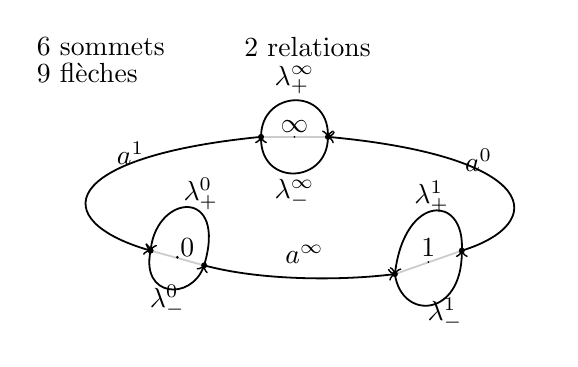
\begin{tikzpicture}[x=.85cm,y=.85cm,line width=.65pt]
\node[anchor=west] at (-.7,4.25) {6 sommets};
\node[anchor=west] at (-.7,3.85) {9 flèches};
\node[anchor=west] at (2.4,4.25) {2 relations};
\draw[gray!40] (2.8,2.9)--(3.8,2.9);
\draw[gray!40] (1.15,1.2)--(1.95,.98);
\draw[gray!40] (4.8,.85)--(5.8,1.2);
\draw[->] (2.8,2.9) .. controls (2.8,3.6) and (3.8,3.65) .. (3.8,2.9);
\draw[->] (3.8,2.9) .. controls (3.8,2.2) and (2.8,2.15) .. (2.8,2.9);
\node at (3.3,3.75) {$\lambda^\infty_+$};
\node at (3.3,2.05) {$\lambda^\infty_-$};
\fill (3.3,2.9) circle (.015); \node at (3.3,3.05) {$\infty$};
\draw[->] (1.95,.98) .. controls (2.3,2.15) and (1.25,2.05) .. (1.15,1.2);
\draw[->] (1.15,1.2) .. controls (1,.5) and (1.75,.45) .. (1.95,.98);
\node at (1.9,2.05) {$\lambda^0_+$}; \node at (1.4,.45) {$\lambda^0_-$};
\fill (1.55,1.1) circle (.022); \node at (1.7,1.25) {$0$};
\draw[->] (5.8,1.2) .. controls (5.85,2.05) and (4.95,2.05) .. (4.8,.85);
\draw[->] (4.8,.85) .. controls (4.9,.15) and (5.8,.2) .. (5.8,1.2);
\node at (5.35,2.0) {$\lambda^1_+$}; \node at (5.55,.25) {$\lambda^1_-$};
\fill (5.3,1.03) circle (.015); \node at (5.3,1.25) {$1$};
\draw[->] (2.8,2.9) .. controls (-.25,2.6) and (-.4,1.65) .. (1.15,1.2);
\node at (.85,2.65) {$a^1$};
\draw[->] (5.8,1.2) .. controls (7.1,1.6) and (7.0,2.6) .. (3.8,2.9);
\node at (6.05,2.55) {$a^0$};
\draw[->] (1.95,.98) .. controls (2.8,.75) and (4,.75) .. (4.8,.85);
\node at (3.45,1.15) {$a^\infty$};
\foreach \x/\y in {2.8/2.9,3.8/2.9,1.15/1.2,1.95/.98,4.8/.85,5.8/1.2} \fill (\x,\y) circle (.045);
\end{tikzpicture}}
&
\figure{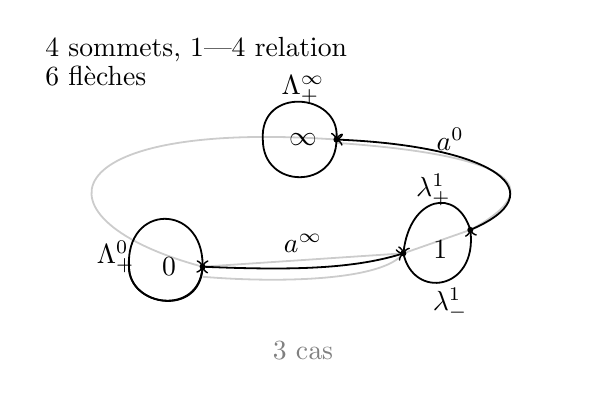
\begin{tikzpicture}[x=.85cm,y=.85cm,line width=.65pt]
\node[anchor=west] at (-.7,4.25) {4 sommets, \unsure{1|4} relation};
\node[anchor=west] at (-.7,3.85) {6 flèches};
\draw[gray!40] (3.8,2.9) .. controls (-.5,3.2) and (-.8,1.7) .. (1.8,1.0);
\draw[gray!40] (1.8,1.0)--(4.8,1.2);
\draw[gray!40] (4.8,1.2)--(5.8,1.55);
\draw[gray!40] (1.8,.85) .. controls (3,.75) and (4.5,.8) .. (4.8,1.2);
\draw[gray!40] (5.8,1.55) .. controls (7.2,2.3) and (6,2.7) .. (3.8,2.85);
\draw[->] (3.8,2.9) .. controls (3.8,2.15) and (2.7,2.15) .. (2.7,2.9) .. controls (2.65,3.7) and (3.85,3.6) .. (3.8,2.9);
\node at (3.3,3.65) {$\Lambda^\infty_+$}; \node at (3.3,2.9) {$\infty$};
\draw[->] (1.8,1.0) .. controls (1.75,.25) and (.7,.4) .. (.7,1.0) .. controls (.65,1.95) and (1.8,1.95) .. (1.8,1.0);
\draw[->] (.7,1.0) .. controls (.7,.4) and (1.75,.25) .. (1.8,1.0);
\node at (.5,1.15) {$\Lambda^0_+$}; \node at (1.3,1.0) {$0$};
\draw[->] (1.8,1.0) .. controls (3.0,.95) and (4,.95) .. (4.8,1.2);
\node at (3.3,1.35) {$a^\infty$};
\draw[->] (5.8,1.55) .. controls (5.6,2.2) and (4.9,2.05) .. (4.8,1.2);
\draw[->] (4.8,1.2) .. controls (4.95,.5) and (5.9,.65) .. (5.8,1.55);
\node at (5.25,2.15) {$\lambda^1_+$}; \node at (5.5,.45) {$\lambda^1_-$}; \node at (5.35,1.25) {$1$};
\draw[->] (5.8,1.55) .. controls (7.1,2.1) and (6.2,2.8) .. (3.8,2.9);
\node at (5.5,2.9) {$a^0$};
\foreach \x/\y in {3.8/2.9,1.8/1,4.8/1.2,5.8/1.55} \fill (\x,\y) circle (.045);
\node[gray] at (3.3,-.25) {3 cas};
\end{tikzpicture}}
\\
\figure{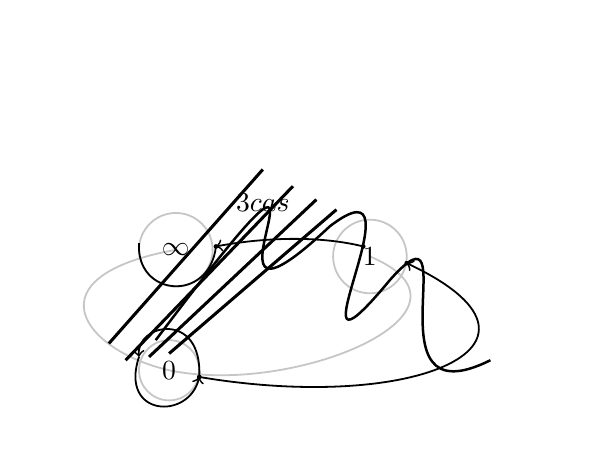
\begin{tikzpicture}[x=.85cm,y=.85cm,line width=.65pt]
\draw[gray!45] (1.2,2.7) circle (.55);
\draw[gray!45] (4.1,2.6) circle (.55);
\draw[gray!45] (1.1,.9) circle (.45);
\draw[gray!45] (1.2,2.7) .. controls (-1,2.3) and (-.2,1.2) .. (1.1,.9) .. controls (3,.5) and (6,1.8) .. (4.1,2.6);
\node at (1.2,2.7) {$\deleted{\infty}$}; \node at (4.1,2.6) {$\deleted{1}$}; \node at (1.1,.9) {$\deleted{0}$};
\draw[->] (4.0,2.75) .. controls (3.4,2.9) and (2.6,2.9) .. (1.8,2.75);
\draw (1.8,2.75) .. controls (1.7,1.9) and (.6,2.0) .. (.65,2.8);
\draw[->] (1.55,.8) .. controls (4.8,.25) and (7.2,1.3) .. (4.65,2.5);
\draw[->] (1.55,.8) .. controls (1.6,1.8) and (.6,1.6) .. (.65,1.1);
\draw[->] (.65,1.1) .. controls (.35,.2) and (1.4,.15) .. (1.55,.8);
\node at (2.5,3.4) {$\deleted{\unsure{3\text{ cas}}}$};
\foreach \x/\y in {1.8/2.75,4/2.75,4.65/2.5,1.55/.8} \fill (\x,\y) circle (.035);
\draw[line width=1.1pt] (.2,1.3)--(2.5,3.9) (.45,1.05)--(2.95,3.65) (.8,1.1)--(3.3,3.45) (1.1,1.15)--(3.6,3.3);
\draw[line width=.9pt] (.9,1.35) .. controls (4.4,6) and (1.0,.7) .. (3.5,3.05) .. controls (5.0,4.2) and (2.7,.2) .. (4.4,2.25) .. controls (5.6,3.6) and (4.0,.1) .. (5.9,1.05);
\end{tikzpicture}}
&
\figure{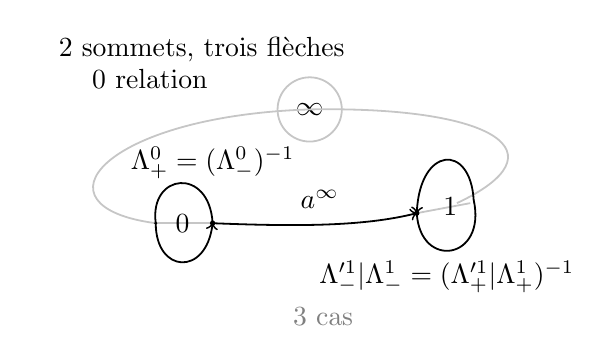
\begin{tikzpicture}[x=.85cm,y=.85cm,line width=.65pt]
\node[anchor=west] at (-.7,3.65) {2 sommets, trois flèches};
\node[anchor=west] at (-.2,3.2) {0 relation};
\draw[gray!45] (3.2,2.75) circle (.48); \node at (3.2,2.75) {$\infty$};
\draw[gray!45] (.9,1.05) .. controls (-1,1.3) and (.1,2.65) .. (3.2,2.75) .. controls (6.0,2.8) and (7.0,2.1) .. (5.4,1.35);
\draw[gray!45] (.9,1.05)--(1.75,1.05); \draw[gray!45] (4.8,1.2)--(5.6,1.35);
\draw[->] (1.75,1.05) .. controls (1.7,1.9) and (.8,1.8) .. (.9,1.05) .. controls (.9,.3) and (1.65,.25) .. (1.75,1.05);
\fill (.9,1.05) circle (.025); \fill (1.75,1.05) circle (.04); \node at (1.3,1.05) {$0$};
\node at (1.75,1.95) {$\Lambda^0_+=(\Lambda^0_-)^{-1}$};
\draw[->] (1.75,1.05) .. controls (3,1.0) and (4,1.0) .. (4.8,1.2);
\node at (3.35,1.4) {$a^\infty$};
\draw[->] (4.8,1.2) .. controls (4.85,.35) and (5.85,.5) .. (5.65,1.4) .. controls (5.6,2.25) and (4.85,2.2) .. (4.8,1.2);
\fill (4.8,1.2) circle (.04); \node at (5.3,1.3) {$1$};
\node at (5.25,.25) {$\unsure{\Lambda^{\prime1}_-|\Lambda^1_-}=(\unsure{\Lambda^{\prime1}_+|\Lambda^1_+})^{-1}$};
\node[gray] at (3.4,-.35) {3 cas};
\end{tikzpicture}}
\\
\figure{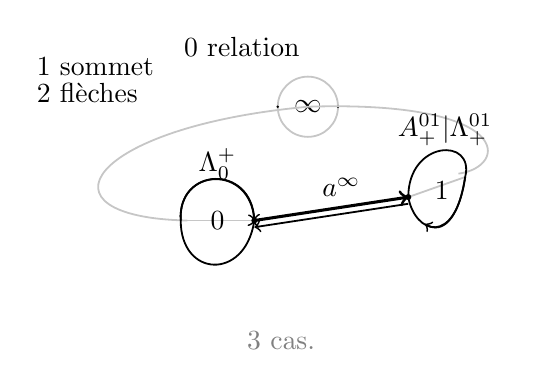
\begin{tikzpicture}[x=.85cm,y=.85cm,line width=.65pt]
\node[anchor=west] at (-.7,3.5) {1 sommet};
\node[anchor=west] at (-.7,3.1) {2 flèches};
\node[anchor=west] at (1.5,3.8) {0 relation};
\draw[gray!45] (3.5,2.9) circle (.45); \node at (3.5,2.9) {$\infty$};
\fill (3.05,2.9) circle (.022); \fill (3.95,2.9) circle (.022);
\draw[gray!45] (1.7,1.2) .. controls (-.65,1.25) and (.2,2.6) .. (3.5,2.9) .. controls (6.6,3) and (6.5,2.0) .. (5.75,1.9);
\draw[gray!45] (1.6,1.2)--(2.7,1.2); \draw[gray!45] (5,1.55)--(5.85,1.85);
\draw[->] (2.7,1.2) .. controls (2.65,2.05) and (1.55,2.0) .. (1.6,1.2) .. controls (1.6,.35) and (2.55,.3) .. (2.7,1.2);
\draw[->] (1.6,1.2) .. controls (1.55,2.0) and (2.65,2.05) .. (2.7,1.2);
\node at (2.15,2.05) {$\Lambda_0^+$}; \node at (2.15,1.2) {$0$};
\draw[->,line width=1.1pt] (2.7,1.2)--(5,1.55);
\draw[->] (5,1.45)--(2.7,1.1);
\node at (4,1.7) {$\deleted{\unsure{a^\infty}}$};
\draw (5,1.55) .. controls (5,2.4) and (6,2.45) .. (5.85,1.85) .. controls (5.7,.8) and (5.1,1.0) .. (5,1.55);
\draw[->] (5.85,1.85) .. controls (5.75,1.2) and (5.5,1.0) .. (5.25,1.15);
\node at (5.55,2.55) {$\unsure{A_+^{01}|\Lambda_+^{01}}$}; \node at (5.5,1.65) {$1$};
\fill (2.7,1.2) circle (.045); \fill (5,1.55) circle (.045);
\node[gray] at (3.1,-.6) {3 cas.};
\end{tikzpicture}}
&
\end{tabular}
\mspage{105}

\scanpage{107}
UNIVERSITE DES SCIENCES

ET TECHNIQUES DU LANGUEDOC

MATHEMATIQUES

24.03.80

\uline{SEMINAIRE D'ALGEBRE}

Vendredi 28.03.1980 à 9 h

Michel COSTE, C.N.R.S., Topologie du spectre réel d'un anneau I.

Vendredi 28.03.1980 à 10 h

Marie-Françoise COSTE, Université de Paris-Nord, Topologie du spectre réel d'un anneau II.

Ces conférences ont lieu en Salle 431 du Bâtiment de Mathématiques.

N.B.\quad 1) La conférence de R. PICCININI initialement prévue pour cette date, a été annulée, à la demande du conférencier.

2) A partir de 11 h en Salle 431, il y aura \unsure{lés|lès|les} soutenances des thèses de 3e cycle de Monsieur BURGUENTO et de Madame ALCALDE.

\uline{Sujet} : Formes sur les algèbres non associatives.

A. MICALI

\mspage{106}

\scanpage{108}

\figure{%
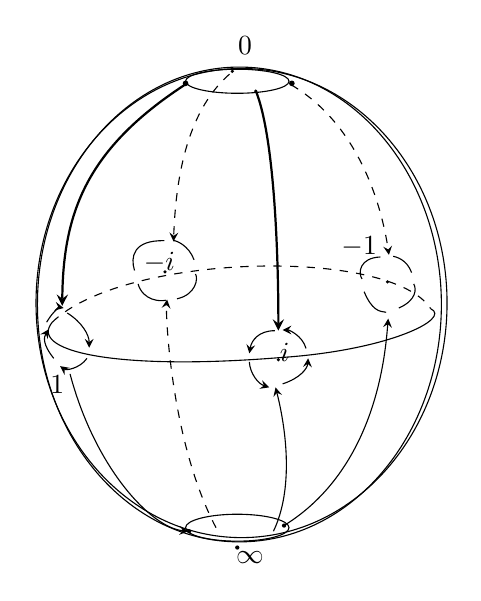
\begin{tikzpicture}[x=0.9cm,y=0.9cm,>=stealth]
\draw[thin] (0,0) ellipse (2.85 and 3.35);
\draw[thin] (0.03,0.02) ellipse (2.9 and 3.31);
\draw (-0.03,3.15) ellipse (0.73 and 0.17);
\draw (-0.03,-3.15) ellipse (0.73 and 0.19);
\node at (0.08,3.65) {$0$};
\node at (0.15,-3.57) {$\infty$};
\draw[dashed] (-2.64,-0.25) .. controls (-1.65,0.72) and (2.13,0.82) .. (2.7,-0.06);
\draw (-2.64,-0.25) .. controls (-2.98,-0.65) and (-1.8,-0.94) .. (0.57,-0.75) .. controls (2.1,-0.65) and (3.0,-0.2) .. (2.7,-0.06);
\draw[->,thick] (-0.77,3.1) .. controls (-2.15,2.2) and (-2.49,1.3) .. (-2.5,-0.02);
\draw[->] (-2.39,-0.98) .. controls (-2.04,-2.3) and (-1.25,-3.15) .. (-0.72,-3.2);
\draw[->,thick] (0.23,3.02) .. controls (0.5,2.35) and (0.55,0.65) .. (0.55,-0.37);
\draw[->] (0.48,-3.2) .. controls (0.76,-2.62) and (0.67,-1.8) .. (0.51,-1.17);
\draw[dashed,->] (-0.14,3.25) .. controls (-0.77,2.7) and (-0.9,1.7) .. (-0.93,0.89);
\draw[dashed,->] (-0.33,-3.15) .. controls (-0.98,-1.91) and (-1.04,-0.1) .. (-1.02,0.07);
\draw[dashed,->] (0.73,3.1) .. controls (1.75,2.5) and (2.03,1.25) .. (2.11,0.7);
\draw[->] (0.63,-3.12) .. controls (1.94,-2.31) and (2.06,-0.68) .. (2.1,-0.2);
\draw[->] (-2.43,-0.12) .. controls (-2.22,-0.25) and (-2.12,-0.43) .. (-2.12,-0.61);
\draw[->] (-2.15,-0.76) .. controls (-2.26,-0.91) and (-2.45,-0.93) .. (-2.53,-0.87);
\draw[->] (-2.62,-0.76) .. controls (-2.78,-0.56) and (-2.76,-0.46) .. (-2.69,-0.35);
\draw[->] (-2.72,-0.25) .. controls (-2.62,-0.08) and (-2.53,-0.04) .. (-2.48,-0.05);
\node at (-2.57,-1.13) {$1$};
\draw[->] (0.5,-0.37) .. controls (0.27,-0.37) and (0.17,-0.51) .. (0.14,-0.69);
\draw[->] (0.14,-0.81) .. controls (0.15,-0.98) and (0.27,-1.12) .. (0.42,-1.17);
\draw[->] (0.61,-1.12) .. controls (0.86,-1.04) and (0.96,-0.9) .. (0.97,-0.76);
\draw[->] (0.94,-0.62) .. controls (0.89,-0.44) and (0.7,-0.36) .. (0.61,-0.36);
\node at (0.64,-0.68) {$i$};
\fill (0.55,-0.78) circle (0.025);
\draw (-1.06,0.9) .. controls (-1.5,0.91) and (-1.54,0.67) .. (-1.48,0.48);
\draw (-1.43,0.29) .. controls (-1.36,0.05) and (-1.11,0.04) .. (-1.04,0.06);
\draw (-0.88,0.08) .. controls (-0.61,0.14) and (-0.58,0.37) .. (-0.62,0.43);
\draw (-0.64,0.63) .. controls (-0.71,0.83) and (-0.9,0.91) .. (-0.93,0.9);
\node at (-1.13,0.59) {$-i$};
\fill (-1.05,0.46) circle (0.025);
\draw (1.99,0.67) .. controls (1.7,0.66) and (1.67,0.45) .. (1.73,0.36);
\draw (1.76,0.18) .. controls (1.87,-0.08) and (1.97,-0.1) .. (2.07,-0.11);
\draw (2.25,-0.05) .. controls (2.5,0.06) and (2.5,0.22) .. (2.46,0.29);
\draw (2.43,0.45) .. controls (2.36,0.64) and (2.21,0.67) .. (2.17,0.68);
\node at (1.69,0.81) {$-1$};
\fill (2.09,0.32) circle (0.025);
\fill (-0.76,3.12) circle (0.04);\fill (0.74,3.12) circle (0.04);
\fill (-0.1,3.29) circle (0.025);\fill (0.23,3.01) circle (0.025);
\fill (-0.71,-3.2) circle (0.03);\fill (0.63,-3.12) circle (0.03);
\fill (-0.03,-3.43) circle (0.03);
\end{tikzpicture}%
}

\diagram{\begin{tikzcd}[ampersand replacement=\&,row sep=small]
z \arrow[r] \& -z \\
z \arrow[r] \& \dfrac{1}{z} \\
\unsure{z} \& {} \arrow[l]
\end{tikzcd}}

\diagram{\begin{tikzcd}[ampersand replacement=\&]
1 \arrow[r] \& \mathbb{F}_2^2 \arrow[r] \& A_4 \arrow[r] \& \mathbb{Z}/3\mathbb{Z} \arrow[r] \& 1
\end{tikzcd}}

\figure{%
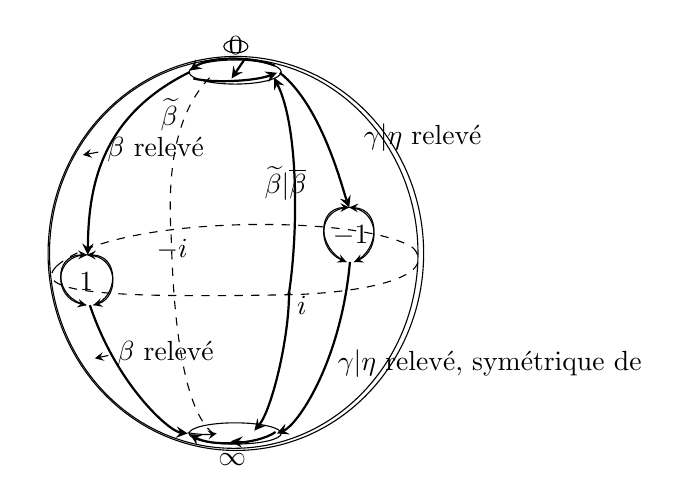
\begin{tikzpicture}[x=0.9cm,y=0.9cm,>=stealth]
\draw[thin] (0,0) ellipse (2.6 and 2.75);
\draw[thin] (0.03,0) ellipse (2.65 and 2.78);
\draw (0.02,2.56) ellipse (0.65 and 0.17);
\draw (0.02,-2.54) ellipse (0.65 and 0.15);
\node at (0.03,2.93) {$\unsure{0}$};
\draw (0.03,2.92) ellipse (0.17 and 0.09);
\node at (-0.02,-2.91) {$\infty$};
\draw[dashed] (-2.5,-0.18) .. controls (-1.7,0.55) and (1.8,0.56) .. (2.53,0.08);
\draw[dashed] (-2.5,-0.18) .. controls (-2.9,-0.58) and (-1.6,-0.63) .. (0.9,-0.58) .. controls (2.2,-0.52) and (2.84,-0.25) .. (2.53,0.08);
\draw[->,thick] (-0.62,2.56) .. controls (-1.9,1.93) and (-2.05,0.91) .. (-2.06,-0.02);
\draw[->,thick] (-2.03,-0.73) .. controls (-1.65,-1.86) and (-0.91,-2.51) .. (-0.65,-2.54);
\draw[->,thick] (0.65,2.55) .. controls (1.25,2.08) and (1.54,0.89) .. (1.63,0.65);
\draw[->,thick] (1.64,-0.12) .. controls (1.51,-1.54) and (0.9,-2.42) .. (0.61,-2.54);
\draw[dashed] (-0.34,2.48) .. controls (-0.93,1.87) and (-0.92,0.84) .. (-0.88,0.18) .. controls (-0.84,-1.3) and (-0.64,-2.26) .. (-0.3,-2.53);
\draw[->] (-0.65,-2.53) .. controls (-0.4,-2.57) and (-0.3,-2.55) .. (-0.24,-2.54);
\draw[->,thick] (0.78,-0.56) .. controls (0.91,0.3) and (0.92,1.78) .. (0.57,2.48);
\draw[->,thick] (0.78,-0.56) .. controls (0.78,-1.22) and (0.53,-2.22) .. (0.29,-2.5);
\draw[->] (-2.07,-0.02) .. controls (-2.55,-0.02) and (-2.55,-0.62) .. (-2.08,-0.73);
\draw[->] (-2.07,-0.02) .. controls (-1.61,-0.03) and (-1.62,-0.62) .. (-1.98,-0.73);
\draw[->] (-2.08,-0.73) .. controls (-2.55,-0.62) and (-2.55,-0.02) .. (-2.07,-0.02);
\draw[->] (-1.98,-0.73) .. controls (-1.62,-0.62) and (-1.61,-0.03) .. (-2.07,-0.02);
\node at (-2.08,-0.39) {$1$};
\draw[->] (1.63,0.65) .. controls (1.17,0.64) and (1.17,0.06) .. (1.59,-0.12);
\draw[->] (1.63,0.65) .. controls (2.08,0.62) and (2.06,0.04) .. (1.7,-0.12);
\draw[->] (1.59,-0.12) .. controls (1.17,0.06) and (1.17,0.64) .. (1.63,0.65);
\draw[->] (1.7,-0.12) .. controls (2.06,0.04) and (2.08,0.62) .. (1.63,0.65);
\node at (1.65,0.25) {$-1$};
\node at (-0.87,0.05) {$-i$};
\fill (0.78,-0.56) circle (0.025);\node at (0.96,-0.73) {$i$};
\node at (-0.91,1.96) {$\widetilde{\beta}$};
\node at (0.73,0.99) {$\unsure{\widetilde{\beta}|\overline{\beta}}$};
\node[anchor=west] at (-1.92,1.46) {$\beta$ relevé};
\draw[->] (-1.91,1.43) -- (-2.13,1.39);
\node[anchor=west] at (-1.78,-1.41) {$\beta$ relevé};
\draw[->] (-1.77,-1.44) -- (-1.96,-1.48);
\node[anchor=west] at (1.7,1.64) {$\unsure{\gamma|\eta}$ relevé};
\node[anchor=west] at (1.33,-1.55) {$\unsure{\gamma|\eta}$ relevé, \unsure{symétrique de}};
\draw[->,thick] (0.58,2.65) .. controls (0.2,2.8) and (-0.36,2.77) .. (-0.62,2.58);
\draw[->,thick] (-0.57,2.47) .. controls (-0.3,2.4) and (0.3,2.43) .. (0.61,2.55);
\draw[->,thick] (0.14,2.72) -- (-0.03,2.47);
\draw[->,thick] (0.59,-2.52) .. controls (0.31,-2.71) and (-0.33,-2.72) .. (-0.62,-2.55);
\draw[->,thick] (0.21,-2.67) -- (-0.04,-2.65);
\end{tikzpicture}%
}

\[
l_{\infty}l_1l_0l_{-1}=1
\]

\mspage{107}

\scanpage{109}

\begin{center}
U N I V E R S I T E\\
DES SCIENCES ET TECHNIQUES\\
DU LANGUEDOC\\
------------
\end{center}

MONTPELLIER, le 06 Octobre 1978

Service de la Scolarité\\
MR / GJ\\
Diffusion\quad : Liste H\\
N° : 5462

\begin{center}
\uline{AVIS DE SOUTENANCE D'UNE THESE DE DOCTORAT D ' ETAT}
\end{center}

\uline{Nom et prénom du candidat} : SOONCKINDT Louis

\uline{Titre de la thèse} : Contribution à l'étude des propriétés électroniques des surfaces réelles et clivées sous ultra-vide d'antimoniure de gallium.

\uline{Date, heure et lieu de soutenance prévus} : 26 OCTOBRE 1978 à 11 Heures\\
Salle de cours n° 7 - U.S.T.L.

\uline{Nom du Directeur de thèse} : Monsieur le Professeur LASSABATERE Louis.

\uline{Désignation du Laboratoire où la thèse est préparée} : C. E. E. S.

\uline{Résumé de la thèse} : Après avoir décrit le montage expérimental réalisé au Laboratoire et permettant l'étude des travaux de sortie par la méthode de Kelvin on étudie les propriétés électroniques des surfaces réelles et des surfaces propres, obtenues par clivage, de GaSb. On précise les interactions entre les états électroniques de surface (\textit{intrinsèques et extrinsèques}) dans l'obscurité et sous éclairement dans la gamme de température comprise entre 100 et $420^\circ$ K.

\uline{Durée approximative des recherches ayant abouti à la thèse} : 8 ans.

\uline{Noms des Rapporteurs} :

\diagram{$\begin{array}{lll}
\text{LASSABATERE} & \text{Louis} & \text{, Professeur, Electronique, U. S. T. L.} \\
\text{LANNOO} & \text{Maurice} & \text{Maître Recherche, Physique du Solide, ISEN LILLE} \\
\text{SEBENNE} & \text{Claude} & \text{Maître Recherche, Physique du Solide, PARIS 6}
\end{array}$}

\uline{Composition du jury proposé} :

\diagram{$\begin{array}{lll}
\text{PISTOULET} & \text{B.} & \text{Professeur, Electronique, U.S.T.L.} \\
 & & \text{Président} \\
\text{LACOSTE} & \text{R.} & \text{Professeur, Electronique, Univers. P. SABATIER, TOULOUSE} \\
\text{LANNOO} & \text{M.} & \text{Maître Recherche, Physique du Solide, ISEN LILLE} \\
\text{SEBENNE} & \text{C.} & \text{Maître Recherche, Physique du Solide, PARIS 6} \\
 & & \text{(Membre extérieur choisi en raison de sa compétence scientifique)} \\
\text{LASSABATERE} & \text{L.} & \text{Professeur, Electronique, U.S.T.L.} \\
\text{NOUGIER} & \text{J.-P.} & \text{Professeur, Electronique, U.S.T.L.} \\
 & & \text{(Membre étranger à la spécialité du candidat).}
\end{array}$}

Le Secrétaire Général,

\figure{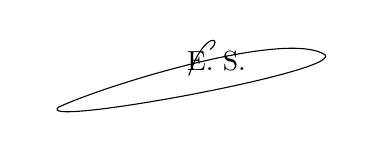
\begin{tikzpicture}[x=1cm,y=1cm]
\node at (0.7,0.33) {\unsure{E. S.}};
\draw (-1.3,-0.25) .. controls (-0.72,0.02) and (1.5,0.71) .. (2.05,0.43) .. controls (2.53,0.24) and (-1.69,-0.53) .. (-1.3,-0.25);
\draw (0.35,0.15) .. controls (0.56,0.75) and (0.8,0.62) .. (0.62,0.48);
\end{tikzpicture}}

\uline{E. S I A U}

MR LE PROFESSEUR GROTHENDIECK A.

\hfill 5

MATHEMATIQUES

\mspage{108}

\scanpage{110}

\diagram{\begin{tikzcd}[ampersand replacement=\&,column sep=large,row sep=large]
\cdot E_0 \arrow[r,dash] \arrow[d] \& \pi_0(E_0)=\deleted{E_0/\pi\,\unsure{\operatorname{Ssgr}}(} \arrow[d] \\
\unsure{\operatorname{Sgr}|\operatorname{Ssgr}}(\pi) \arrow[r,Rightarrow] \& \operatorname{Ssgr}(\unsure{\Pi|E})/\pi
\end{tikzcd}}
\[
\underbrace{\hspace{6em}}_{\unsure{E|\mathcal{B}}_0\ \text{pris ci-dessus}}
\]

\margin{$\mathcal{E}/\pi=\Gamma$}

\diagram{\begin{tikzcd}[ampersand replacement=\&,column sep=large,row sep=small]
\mathcal{E}(=\Gamma.\unsure{\Pi|\pi}) \& \& \unsure{\mathcal{E}} \arrow[d] \\
\bigcup \& \& {} \\
\pi \arrow[r,dash] \& E_0 \arrow[r,Rightarrow] \& \operatorname{Ssgr}(\pi)/\pi
\end{tikzcd}}

\figure{%
\begin{tikzpicture}[x=0.8cm,y=0.8cm,>=stealth]
\begin{scope}[rotate=180,transform shape]
\begin{scope}[shift={(0,0)}]
\draw (0,0) ellipse (1.65 and 1.75);
\draw[thin] (0.03,0) ellipse (1.68 and 1.72);
\draw (0,1.7) ellipse (0.28 and 0.08);\draw (0,-1.7) ellipse (0.28 and 0.1);
\fill (0,1.7) circle (0.045);\fill (0,-1.7) circle (0.04);
\node at (0,2.03) {$0$};\node at (0,-2.02) {$\infty$};
\draw (0,0) ellipse (1.64 and 0.27);
\draw[->,thick] (-0.1,-1.64) .. controls (-0.18,-0.3) and (-0.05,1.2) .. (0,1.65);
\draw[dashed] (0.08,1.6) .. controls (0.12,0.6) and (0.13,-0.6) .. (0.02,-1.6);
\draw[->] (-0.12,1.63) .. controls (-1.35,1.45) and (-1.6,-0.6) .. (-0.1,-1.67);
\draw[->] (0.17,-1.65) .. controls (1.37,-1.5) and (1.5,0.8) .. (0.17,1.65);
\draw[dashed,->] (-0.23,1.65) .. controls (-1.8,1.1) and (-1.73,-1) .. (-0.14,-1.65);
\draw[dashed,->] (0.28,-1.65) .. controls (1.8,-1.1) and (1.78,1.1) .. (0.29,1.64);
\draw (-0.63,0.27) circle (0.19);\fill (-0.63,0.27) circle (0.025);
\draw (0.65,0.28) circle (0.19);\fill (0.65,0.28) circle (0.025);
\draw (-0.55,-0.2) circle (0.2);\fill (-0.55,-0.2) circle (0.025);
\draw (0.62,-0.17) circle (0.19);\fill (0.62,-0.17) circle (0.025);
\draw (-1.65,0.02) ellipse (0.1 and 0.19);\draw (1.64,0.07) ellipse (0.1 and 0.17);
\node at (1.98,0.11) {$1$};
\node at (0.29,1.47) {$a$};\node at (-0.2,0.65) {$c$};\node at (-0.32,-0.28) {$b$};
\node at (-0.55,-0.01) {$\unsure{a}$};
\node at (0.64,1.86) {$\deleted{\unsure{R\to a}}$};
\draw[thick] (0.36,1.78) -- (0.84,1.95);
\end{scope}
\draw[->] (-1.5,-2.1) -- (-2.2,-4.15);
\draw[->] (-0.7,-2.02) -- (-1.35,-3.95);
\node[anchor=west,align=left] at (-0.78,-3.15) {division\\par $D$\\\unsure{ramification}\\\unsure{en les} $P_{\unsure{\omega}}$\\$Q_a,\ R_s$};

\begin{scope}[shift={(5,-0.5)}]
\draw (0,0) circle (1.85);\draw[thin] (0.02,0.01) circle (1.88);
\draw (0,0) ellipse (1.83 and 0.38);
\draw (0,1.83) ellipse (0.32 and 0.1);\draw (0,-1.8) ellipse (0.37 and 0.12);
\fill (0,1.83) circle (0.035);\fill (0,-1.8) circle (0.035);
\node at (0,2.15) {$\infty$};\node at (0,-2.08) {$0$};
\draw[->] (-0.15,1.8) .. controls (-1.58,1.56) and (-2.05,-0.8) .. (-0.2,-1.8);
\draw[->] (-1.81,0.08) .. controls (-0.8,0.51) and (0.8,0.54) .. (1.75,0.18);
\draw[->] (-1.81,-0.06) .. controls (-0.75,-0.46) and (0.9,-0.47) .. (1.74,-0.12);
\draw (1.78,0.04) ellipse (0.13 and 0.25);\draw[->] (1.76,-0.19) arc (-95:240:0.13 and 0.24);
\node at (2.01,0.04) {$1$};
\draw[->] (1.83,0.2) .. controls (1.76,1.0) and (1.25,1.66) .. (0.25,1.83);
\draw[->] (1.83,-0.2) .. controls (1.7,-1.1) and (0.99,-1.68) .. (0.2,-1.8);
\end{scope}
\draw[->] (2.55,-0.4) -- (4.05,-3.53);
\node[anchor=west,align=left] at (2.72,-2.2) {division\\par $D^+$\\(\unsure{ramification seulement en} $\unsure{0},\infty$)};

\begin{scope}[shift={(5,-5.25)}]
\draw[thin] (0,0) circle (1.95);
\draw[thin] (0.02,-0.01) circle (1.98);
\draw (0,0) ellipse (1.94 and 0.43);
\draw[thick] (0,1.9) ellipse (0.47 and 0.12);\draw[thick] (0,-1.9) ellipse (0.48 and 0.12);
\node at (0,2.18) {$0$};\node at (0,-2.2) {$\infty$};
\draw[->,dashed] (-0.18,1.87) .. controls (-0.85,1.3) and (-0.96,0.75) .. (-1.01,0.25);
\draw[->,dashed] (-1.01,-0.33) .. controls (-0.88,-1.05) and (-0.5,-1.7) .. (-0.25,-1.9);
\fill (-1.01,0.25) circle (0.04);
\draw[->,thick] (-1.01,0.25) .. controls (0.15,0.51) and (1.83,0.4) .. (1.81,0.03) .. controls (1.8,-0.12) and (1.55,-0.21) .. (1.37,-0.22);
\draw[->,thick] (-1.01,-0.34) .. controls (-0.27,-0.44) and (0.28,-0.42) .. (0.88,-0.39);
\draw[thick] (1.13,-0.34) circle (0.31);
\draw[->] (0.85,-0.19) arc (150:340:0.31);
\node at (1.13,-0.34) {$1$};
\node at (-1.22,0.4) {$-1$};\node at (-0.83,0.12) {$Q_1$};
\node at (-1.23,1.13) {$b_1^+$};\node at (-1.1,-1.1) {$b_1^-$};
\node at (0.43,0.71) {$d_{\unsure{i|1}}^+(c_{\unsure{i|1}}^+)^{-1}$};
\node at (0.02,-0.18) {$d_{\unsure{i|1}}^-(c_{\unsure{i|1}}^-)^{-1}$};
\node at (1.06,0.23) {$\unsure{(a_{\unsure{i|1}}^{--}a_{\unsure{i|1}}^{-+})}$};
\node at (1.02,-0.89) {$a_{\unsure{i|1}}^{++}\ a_{\unsure{i|1}}^{+-}$};
\node at (1.84,-0.06) {$S_{\unsure{i|1}}^+$};\node at (0.72,-0.27) {$S_{\unsure{i|1}}^-$};
\node at (0.32,0.5) {$i$};\node at (-1.5,-0.6) {$-i$};
\draw[thin] (-2.8,0.78) -- (2.5,-0.88);
\node at (1.57,-0.57) {$\unsure{q}$};
\node at (0.3,1.61) {$a_\infty^+\ a_\infty^-$};
\node at (-0.03,1.96) {$\deleted{\unsure{R_\infty^-}}$};
\node at (-0.03,-1.63) {$R_\infty^+$};
\node at (0.94,-1.95) {$a_\infty^-\ a_\infty^+$};
\draw[->] (-0.42,-1.92) .. controls (-0.1,-2.04) and (0.2,-2.03) .. (0.44,-1.91);
\draw[->,dashed] (0.38,-1.88) -- (-0.18,-1.86);
\draw[->,thick] (1.9,-0.3) .. controls (2.32,-0.22) and (2.37,0.16) .. (2.04,0.29);
\end{scope}

\begin{scope}[shift={(4.85,-9.9)}]
\draw[thin] (0,0) circle (1.72);\draw[thin] (0.03,0.01) circle (1.76);
\draw[thin] (-1.53,0.07) .. controls (-0.75,0.19) and (0.63,0.28) .. (1.5,0.1);
\draw[thin] (-1.5,-0.48) .. controls (-0.57,-0.6) and (0.5,-0.51) .. (1.5,-0.29);
\draw[dashed] (0,1.7) .. controls (-1.23,1.55) and (-1.4,0.87) .. (-1.43,0.16);
\draw[dashed] (-1.43,-0.52) .. controls (-1.14,-1.37) and (-0.53,-1.66) .. (0,-1.7);
\draw[->,thick] (0,1.7) .. controls (1.16,1.57) and (1.44,0.63) .. (1.47,0.01);
\draw[->,thick] (0,-1.7) .. controls (1.02,-1.7) and (1.44,-0.96) .. (1.47,-0.58);
\fill (0,1.7) circle (0.04);\fill (0,-1.7) circle (0.04);
\node at (0,2.01) {$\unsure{-\overline{\xi}|-\xi}$};
\node at (0,-2.02) {$\unsure{-\xi|-\overline{\xi}}$};
\node at (-1.05,1.1) {$c_{\unsure{i|1}}^+$};\node at (-1.01,-1.14) {$c_{\unsure{i|1}}^-$};
\node at (1.21,1.1) {$d_{\unsure{i|1}}^+$};\node at (1.09,-1.27) {$d_{\unsure{i|1}}^-$};
\draw[thick] (1.48,-0.29) ellipse (0.27 and 0.3);
\node at (1.46,-0.3) {$i$};
\node at (1.66,0.06) {$S_{\unsure{i|1}}^+$};\node at (1.65,-0.63) {$S_{\unsure{i|1}}^-$};
\node at (1.96,0.1) {$a_{\unsure{i|1}}^{++}$};\node at (2,-0.21) {$a_{\unsure{i|1}}^{+-}$};
\node at (1.05,-0.02) {$a_{\unsure{i|1}}^{-+}$};\node at (1,-0.54) {$a_{\unsure{i|1}}^{--}$};
\fill (-1.42,0.15) circle (0.04);\node at (-1.29,0.35) {$-1$};\node at (-1.7,0.39) {$Q_1$};
\draw[->,thick] (-1.4,0.15) -- (-0.37,0.22);
\draw[thick] (-0.07,0.22) circle (0.3);\node at (-0.06,0.27) {$\infty$};\fill (-0.1,0.11) circle (0.025);
\node at (-0.45,0.01) {$R_\infty^+$};\node at (-0.85,0.46) {$b_{\unsure{i|1}}^-$};
\draw[->,thick] (-1.4,0.15) .. controls (-1.95,0.05) and (-1.9,-0.28) .. (-1.52,-0.36);
\draw[thick] (-1.25,-0.44) circle (0.24);\node at (-1.25,-0.41) {$0$};
\fill (-1.29,-0.6) circle (0.04);\node at (-1.75,-0.47) {$R_0$};
\node at (-1.9,0.05) {$b_{\unsure{i|1}}^+$};
\draw[thick] (-1.87,-1.2) -- (-1.93,-1.6) -- (-1.59,-1.48) -- (-1.58,-1.17);
\node[anchor=west,align=left] at (2.35,-0.17) {\margin{\unsure{stable} par\\symétrie\\\unsure{autour} de\\l'axe}};
\end{scope}

\begin{scope}[shift={(-0.4,-7.8)}]
\draw (0,0) circle (1.28);\draw[thick] (0.03,0.02) circle (1.29);
\draw[thick] (0,-0.05) ellipse (1.3 and 0.27);
\draw (-0.95,-0.15) circle (0.15);\draw (0.98,-0.1) circle (0.15);\draw (0,0.2) circle (0.17);
\node at (-0.93,-0.42) {$\deleted{\unsure{0}}$};\node at (1.01,-0.33) {$\deleted{\unsure{1}}$};\node at (0,0.23) {$\deleted{\unsure{\infty}}$};
\fill (0,-0.84) circle (0.03);\node at (0.18,-0.85) {$\deleted{\unsure{0}}$};
\draw (-0.4,1.23) .. controls (-1.05,0.7) and (-0.94,-0.9) .. (-0.09,-1.23);
\draw (0.5,1.17) .. controls (0.85,0.4) and (0.66,-0.8) .. (0.1,-1.2);
\draw[thick] (-1.43,-0.36) -- (0.27,1.49) -- (-0.2,-0.89) -- (0.79,1.21) .. controls (1.4,1.4) and (0.8,-0.6) .. (0.2,-1.4);
\draw (-0.95,-1.1) .. controls (-0.7,1.4) and (1.2,1.4) .. (0.66,-1.35);
\end{scope}
\begin{scope}[shift={(-0.65,-10.2)}]
\draw (0,0) circle (1.48);\draw (0,0.12) ellipse (1.47 and 0.28);
\fill (-0.8,-0.05) circle (0.035);\node at (-0.84,-0.24) {$\deleted{0}$};
\fill (0.08,0.39) circle (0.035);\node at (0.11,0.59) {$\deleted{\infty}$};
\fill (1.14,0.08) circle (0.035);\node at (1.29,0.04) {$\deleted{1}$};
\draw (-0.8,-0.05) -- (0.08,0.39) -- (1.14,0.08) -- cycle;
\draw[thin] (-0.68,0.01) -- (0.09,0.31);\draw[thin] (-0.56,0.04) -- (0.1,0.25);\draw[thin] (-0.4,0.08) -- (0.1,0.2);
\draw[thin] (0.12,0.3) -- (1.0,0.1);\draw[thin] (0.2,0.27) -- (1.08,0.08);
\draw (-1.02,-1.05) .. controls (-0.2,-0.88) and (0.35,0.1) .. (1.1,1.0);
\draw[dashed] (-0.94,-1.16) -- (0.65,0.9);
\draw[thick] (-1.5,-1.7) -- (1.29,1.1);
\draw (-1.09,-1.07) .. controls (-0.8,-0.56) and (0.8,-0.7) .. (0.88,-1.02) .. controls (0.1,-1.43) and (-0.92,-1.24) .. (-1.09,-1.07);
\draw (-0.9,-0.9) .. controls (-0.5,-2) and (0.15,-0.4) .. (0.5,-1.7);
\end{scope}
\draw[->,thick] (3.1,-7.04) -- (1.1,-8.9);
\node[align=left] at (1.8,-7.73) {$0,\infty\longrightarrow\infty$\\$1\longmapsto0$\\$-1\longmapsto1$};
\end{scope}
\end{tikzpicture}%
}

\mspage{109}

\scanpage{111}

\[
\Sigma_J=\mathbb{P}(W(J))\simeq\check{\mathbb{P}}(V(J))
\]
\diagram{\begin{tikzcd}[ampersand replacement=\&]
\unsure{\cdot|0} \arrow[r,dash] \& V(J) \arrow[r] \& \mathcal{O}^J \arrow[r,"\text{somme}"'] \& \mathcal{O} \arrow[r] \& 0
\end{tikzcd}}

\deleted{suite}
\diagram{\begin{tikzcd}[ampersand replacement=\&]
0 \arrow[r] \& F \arrow[r] \& V(J)_\Sigma \arrow[r] \& \mathcal{O}_\Sigma(1) \arrow[r,dash] \& 0
\end{tikzcd}}

\[
F(1)\simeq\mathcal{O}(\omega)
\qquad
(\mathcal{O}\ \text{tordu par }\underline{\omega}=\underline{\omega}(J)\unsure{\,\},}\ \text{i.e. }\det V(J))
\]
\inserted{et}
\[
\mathcal{O}(1)\simeq\check{F}(\omega)
\qquad
\left(\text{par }F\wedge\mathcal{O}_\Sigma(1)
\mathrel{\mathop{\simeq\!\longrightarrow}\limits_{\text{prod. ext.}}}
\det V(J)_\Sigma\simeq\mathcal{O}_\Sigma(\omega)\deleted{\unsure{\Sigma}}\right)
\]
\margin{attention signes!}

\margin{%
$F\times V(J)\longrightarrow\underline{\mathcal{O}}$

Accouplement donné (\deleted{\unsure{fixant|défini par}} un ordre circulaire \unsure{fixé} \deleted{\unsure{en prenant}} $(i,j,k)$), par
$x\wedge y\wedge e_i=x\wedge y\wedge e_j=x\wedge y\wedge e_k$
où $x\in F$, $y\in V(J)$ \unsure{mod} $F$
i.e. donné par \unsure{les mineurs|les 2 mineurs} de la matrice de $(x,y)$.
}

\[
\Omega^1_\Sigma\deleted{\unsure{0}}\simeq F(-1)\simeq\mathcal{O}(\unsure{-2})(\underline{\omega})
\]
\[
\check{\Omega}^1_\Sigma\simeq\mathcal{O}(2)(\underline{\omega})
\qquad\text{fibré tangent à }\Sigma
\]

\margin{$\deleted{\unsure{\varphi_{ij}+\varphi_{jk}+\varphi_{ki}=0}}$}

Points $R_i$ \inserted{\figure{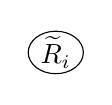
\begin{tikzpicture}[baseline=(r.base)]\node (r) at (0,0) {$\widetilde{R}_i$};\draw (0,0) ellipse (0.35 and 0.27);\end{tikzpicture}}} $(i\in J)$ (``trous'') de $\Sigma$ et $P\Sigma$

\[
\begin{gathered}
R_i\subset\unsure{V|W}(J)\\
\Vert\\
\mathcal{O}_{\unsure{\Sigma}}(e_k-e_j)\\
\simeq\mathcal{O}(\underline{\omega})
\end{gathered}
\qquad\mathcal{O}(1)_{R_i}\simeq\mathcal{O}
\]
\unsure{en associant} à $e_k-e_j$ l'orientation $(i,j,k)$

\margin{%
$\widetilde{R}_i$ pt au-dessus de $R_i$
image de $e_i-e_j=\varphi_{ji}$
$(\equiv e_i-e_k)$ dans $V(J)/R_i$
}

\deleted{Points \unsure{les} $\widetilde{R}_i$ de $P\Sigma_J=\check{V}^{*}(\mathcal{O}_\Sigma(1))$ l'élément $1$ au-dessus de $R_i$.}

\[
\Gamma(\Sigma_{\deleted{\unsure{J}}},\mathcal{O}_\Sigma(1))\simeq V(J)
\]
\deleted{$e_j-e_k$ section $\unsure{\omega_{j,k}}$}
\[
\varphi_{jk}=e_k-e_j\in\Gamma(\Sigma,\mathcal{O}_\Sigma(1))
\]
nulle en $R_i$
\[
\varphi_{kj}=-\varphi_{jk}\qquad\varphi_{jk}(R_i)=0
\]
\margin{$\varphi_{ij}+\varphi_{jk}+\varphi_{ki}=0$.}
\[
\boxed{\varphi_{jk}(R_k)=\widetilde{R}_k\quad\varphi_{jk}(R_j)=-\widetilde{R}_j}
\]
\margin{attention signes!}

Points $Q_i$ $(i\in J)$, $Q_i^\omega{}_{\deleted{\unsure{\omega}}}$ $(i\in J,\omega\in\underline{\omega})$

\[
\begin{gathered}
Q_i\subset\unsure{V|W}(J)\\
\Vert\\
\mathcal{O}(-2e_i+\deleted{\unsure{0|1}}(e_j+e_k))
\end{gathered}
\qquad\mathcal{O}(1)_{Q_i}\simeq\mathcal{O}(\underline{\omega})
\]

\margin{%
les deux points privilégiés de $\mathcal{O}(1)_{Q_i}^{*}$,
induits par $\underline{\omega}$ sont notés $\widetilde{Q}_i$, $\widetilde{Q}'_i$,
ou $Q_{i,\omega}$ $((i,\omega)\in J\times\underline{\omega})$
}

\inserted{%
$(e_i-e_j=\unsure{e_{\omega^2i}-e_{\omega i}})$
classe de \deleted{$\unsure{V(J)}$} dans $V(J)\ \text{mod }Q_i$
}

\deleted{\unsure{par} $\varphi_{\omega i,\omega^2i}(Q_i)=$}

\[
\boxed{Q_i^\omega{}_{\deleted{\unsure{\omega}}}=
\deleted{\unsure{\varphi_{i,\omega i}}}\inserted{\varphi_{\omega i,i}}
\deleted{\unsure{\varphi_{i,\omega^2i}}}(Q_i)}
\]

\margin{NB $\boxed{Q_i^{\omega^{-1}}{}_{\deleted{\unsure{\omega}}}=-Q_i^\omega{}_{\deleted{\unsure{\omega}}}}$

$\varphi_{\omega i,\omega^2i}(Q_i)=2Q_i^\omega{}_{\deleted{\unsure{\omega}}}$}

donc
\[
\widetilde{Q}_i=\varphi_{jk}(Q_i),\quad
\widetilde{Q}'_i=-\varphi_{jk}(Q_i)=\varphi_{kj}(Q_i)
\]

Points $P_\omega$ $(\omega\in\unsure{\underline{\omega}_J|\underline{\omega}})$,
$P_i^\omega{}_{\deleted{\unsure{\omega}}}$ $(i\in J,\omega\in\omega)$.
Soit $\zeta$ une \deleted{\unsure{racine}} racine primitive cubique de $1$ (on prendra
\[
\zeta=\exp\frac{2i\pi}{3}
\]
alors

\mspage{110}

\scanpage{112}

Carte régulière (orientée)\\
du polygône régulier $P_n$ $(n\geq2)$

en le trouant en les sommets et les centres des faces \uline{et} les milieux des segments

\[
\Sigma_n^{\substack{*\\*}*}
=\Sigma_n\setminus\bigl(S(\Sigma_{\unsure{n}})\cup A(\Sigma_{\unsure{n}})\cup F(\Sigma_n)\bigr)
\]
\margin{sommets}
\margin{centres faces}
\margin{milieux arêtes}

\unsure{diviser} par $D_n^+\subset D_{2n}^+$

\diagram{\begin{tikzcd}[ampersand replacement=\&,column sep=large,row sep=small]
\Sigma_n^{\substack{*\\*}*}
 \arrow[r,"\deg n"] \arrow[dddd,phantom,"\simeq" description]
 \& \Sigma_1^{\substack{*\\*}*}=\mathbb{P}_1\setminus\{\underbrace{0,\infty}_{\text{``pôles''}},1,-1\}
 \arrow[r,"\deg2"]
 \& \Sigma_3^{\substack{*\\\cdot}\cdot}=U_{0\,3} \\
 \& \Vert \& \\
 \& \Sigma_n^{\substack{*\\*}*}/D_n \& \\
 \& \Vert \& \\
\Sigma_{2n}^{\substack{*\\*}\unsure{\cdot}}
 \arrow[r]
 \& \Sigma_2^{\substack{*\\*}\cdot}\arrow[r,"2"]
 \& \Sigma_1^{\substack{*\\*}\cdot}\simeq U_0^3
\end{tikzcd}}

\margin{division \deleted{\unsure{par le}} par $D_n/D_n^+$}
\margin{(carte régulière $\overline{\Sigma}_{\unsure{a|n}}$ \unsure{à deux sommets|à deux arêtes})}

division par $D_{2n}^+$

\margin{%
\figure{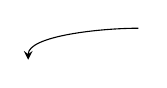
\begin{tikzpicture}[>=stealth]\draw[->] (1.4,0.4) .. controls (0.9,0.4) and (0,0.3) .. (0,0);\end{tikzpicture}}
(on n'a enlevé que les sommets et centres faces)

À cause de cet isomorphisme, on fait \deleted{$\unsure{D_n}$} $D_{2n}$ opérer sur
$\Sigma_n^{\substack{*\\*}*}(\simeq\Sigma_{2n}^{\substack{*\\*}\cdot})$, on peut

donc
}

\diagram{\begin{tikzcd}[ampersand replacement=\&,column sep=large,row sep=large]
 \& \begin{gathered}\Sigma_n^{\substack{*\\*}*}\\\simeq\Sigma_{2n}^{\substack{*\\*}\cdot}\end{gathered}
 \arrow[dl]\arrow[dr] \& \\
\Sigma_{2n}^{\substack{*\\*}\cdot}/D_{2n}^+\arrow[dd]
 \& \& \Sigma_n^{\substack{*\\*}*}/D_n^+\arrow[ll]\arrow[dl] \\
 \& \Sigma^{\substack{*\\*}*}/D_n\arrow[dl,bend left=12] \& \\
\Sigma_{2n}^{\substack{*\\*}\cdot}/D_{2n} \& \&
\end{tikzcd}}

\figure{\begin{tikzpicture}[>=stealth]\draw[->] (0,0) .. controls (0.8,0) and (1.4,0.2) .. (1.6,0.8);\end{tikzpicture}}

\diagram{\begin{tikzpicture}\node (d) at (0,0) {\begin{tikzcd}[ampersand replacement=\&,column sep=large,row sep=large]
 \& \Sigma_n^{\substack{*\\*}*}\simeq\Sigma_{2n}^{\substack{*\\*}\cdot}\arrow[d] \& \\
 \& \Sigma_n^{\substack{*\\*}*}/D_n^+\simeq\Sigma_1^{\substack{\unsure{*}\\*}*}\simeq\Sigma_2^{\substack{*\\*}\cdot}\arrow[dl]\arrow[dr] \& \\
\Sigma^{\substack{*\\*}*}/D_{2n}^+\arrow[dr] \& \& \Sigma_n^{\substack{*\\*}*}/D_n\arrow[dl,dash] \\
 \& \Sigma_n^{\substack{*\\*}\cdot}/D_{2n} \&
\end{tikzcd}};\draw[rounded corners=22pt] (d.south west) rectangle (d.north east);\end{tikzpicture}}

\diagram{\begin{tikzcd}[ampersand replacement=\&]
\Sigma_n^{\substack{*\\*}\cdot}\arrow[r,"D_n^+"] \& \Sigma_1^{\substack{*\\*}\cdot}\simeq U_0^3
\end{tikzcd}}

Si on divise par $D_n$ \deleted{tout} entier, on trouve des ramifications sur les arêtes

\mspage{111}

\scanpage{113}

\figure{%
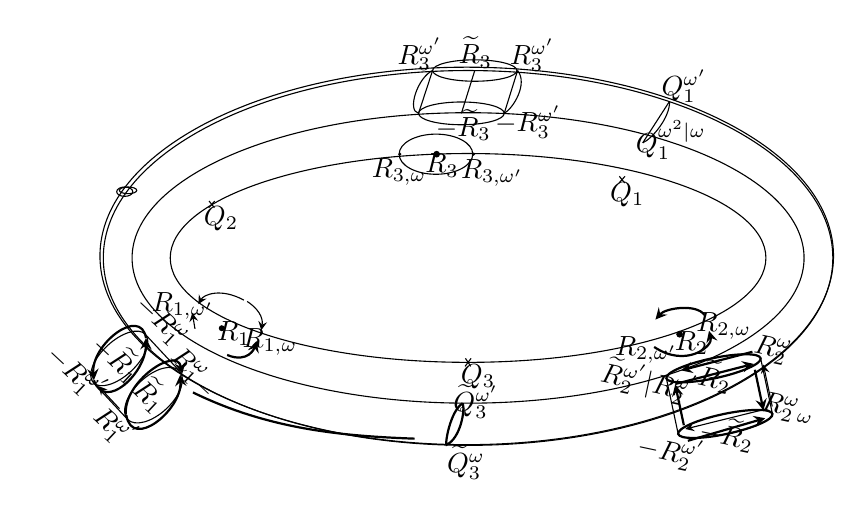
\begin{tikzpicture}[x=0.85cm,y=0.85cm,>=stealth]
\draw[thin] (0,0) ellipse (5.45 and 2.8);
\draw[thin] (-0.02,0.03) ellipse (5.48 and 2.82);
\draw[thin] (0,0) ellipse (5.02 and 2.17);
\draw[thin] (0,0) ellipse (4.45 and 1.56);
\draw[thick] (-4.11,-2.01) .. controls (-2.98,-2.56) and (-1.9,-2.66) .. (-0.8,-2.7);
\fill (-0.47,1.55) circle (0.05);\node at (-0.39,1.38) {$R_3$};
\draw[thin] (-0.48,1.55) ellipse (0.55 and 0.3);
\fill (-1.02,1.55) circle (0.025);\fill (0.08,1.55) circle (0.025);
\node at (-1.03,1.28) {$R_{3,\omega}$};\node at (0.36,1.27) {$R_{3,\omega'}$};
\draw[thin] (0.1,2.8) ellipse (0.63 and 0.16);
\draw[thin] (-0.1,2.16) ellipse (0.64 and 0.17);
\draw[thin] (-0.53,2.8) -- (-0.74,2.16);\draw[thin] (0.74,2.8) -- (0.54,2.16);
\draw[thin] (0.1,2.8) -- (-0.1,2.16);
\draw[thin] (-0.53,2.8) .. controls (-0.75,2.7) and (-0.92,2.2) .. (-0.74,2.16);
\draw[thin] (0.74,2.8) .. controls (0.9,2.6) and (0.67,2.23) .. (0.54,2.16);
\node at (0.11,3.07) {$\widetilde{R}_3$};\node at (-0.07,1.99) {$-\widetilde{R}_3$};
\node at (-0.72,3.04) {$\unsure{R_3^{\omega'}}$};\node at (0.96,3.03) {$\unsure{R_3^{\omega'}}$};
\node at (0.9,2.03) {$-R_3^{\omega'}$};
\draw[thin] (3.01,2.34) .. controls (3.02,2.1) and (2.75,1.78) .. (2.61,1.72);
\draw[thin] (3.01,2.34) -- (2.61,1.72);
\node at (3.23,2.57) {$Q_1^{\omega'}$};\node at (3.03,1.76) {$Q_1^{\unsure{\omega^2|\omega}}$};
\draw (2.3,1.17) ++(-0.045,-0.05) -- ++(0.09,0.1);\draw (2.3,1.17) ++(-0.04,0.05) -- ++(0.08,-0.1);
\node at (2.38,0.95) {$Q_1$};
\draw (-3.83,0.8) ++(-0.045,-0.05) -- ++(0.09,0.1);\draw (-3.83,0.8) ++(-0.04,0.05) -- ++(0.08,-0.1);
\node at (-3.69,0.59) {$Q_2$};
\draw[thin] (-5.08,1.01) ellipse (0.13 and 0.05);
\draw[thin] (-5.13,0.99) ellipse (0.12 and 0.07);
\draw (0,-1.56) ++(-0.045,-0.06) -- ++(0.09,0.12);\draw (0,-1.56) ++(-0.04,0.06) -- ++(0.08,-0.12);
\node at (0.15,-1.78) {$Q_3$};
\draw[thick] (-0.08,-2.17) .. controls (-0.27,-2.29) and (-0.35,-2.79) .. (-0.32,-2.79) .. controls (-0.12,-2.7) and (-0.04,-2.28) .. (-0.08,-2.17);
\node at (0.12,-2.15) {$\widetilde{Q}_3^{\omega'}$};\node at (-0.03,-3.06) {$\unsure{\widetilde{Q}_3^{\omega}}$};
\begin{scope}[shift={(-3.68,-1.05)}]
\fill (0,0) circle (0.045);\node at (0.18,-0.08) {$R_1$};
\draw[->] (0.33,0.42) .. controls (-0.02,0.61) and (-0.27,0.5) .. (-0.35,0.36);
\draw[->] (0.38,0.4) .. controls (0.62,0.24) and (0.61,0.09) .. (0.59,-0.03);
\draw[->,thick] (0.08,-0.4) .. controls (0.4,-0.53) and (0.49,-0.29) .. (0.52,-0.19);
\draw[->] (-0.4,-0.01) -- (-0.44,0.23);
\node at (-0.58,0.33) {$R_{1,\omega'}$};\node at (0.72,-0.21) {$R_{1,\omega}$};
\end{scope}
\begin{scope}[shift={(-4.7,-2.05)},rotate=43]
\draw[thin] (0,0) ellipse (0.53 and 0.28);\draw[thin] (0,0.75) ellipse (0.53 and 0.26);
\draw[thin] (-0.53,0) -- (-0.53,0.75);\draw[thin] (0.53,0) -- (0.53,0.75);
\draw[->,thick] (-0.5,0.06) .. controls (-0.8,-0.39) and (0.16,-0.45) .. (0.5,-0.05);
\draw[->,thick] (-0.5,0.07) .. controls (-0.19,0.46) and (0.76,0.3) .. (0.53,-0.06);
\draw[->,thick] (-0.5,0.77) .. controls (-0.7,0.31) and (0.14,0.32) .. (0.5,0.7);
\draw[->,thick] (0.5,0.7) .. controls (0.77,1.11) and (-0.17,1.19) .. (-0.5,0.77);
\draw[->] (-0.51,0.2) -- (-0.51,0.66);
\node[rotate=-43] at (-0.02,0.03) {$\widetilde{R}_1$};\node[rotate=-43] at (0,0.77) {$-\widetilde{R}_1$};
\node[rotate=-43] at (-0.74,0.05) {$R_1^{\omega'}$};\node[rotate=-43] at (0.67,-0.18) {$R_1^\omega{}_{\deleted{\unsure{-}}}$};
\node[rotate=-43] at (-0.61,1.04) {$-R_1^{\omega'}$};\node[rotate=-43] at (0.82,0.73) {$-R_1^\omega$};
\end{scope}
\begin{scope}[shift={(3.16,-1.14)}]
\fill (0,0) circle (0.05);\node at (0.18,-0.13) {$R_2$};
\draw[->,thick] (0.37,0.29) .. controls (0.25,0.46) and (-0.21,0.39) .. (-0.36,0.22);
\draw[->,thick] (-0.38,-0.19) .. controls (0.1,-0.51) and (0.5,-0.18) .. (0.44,0.05);
\node at (-0.5,-0.23) {$R_{2,\omega'}$};\node at (0.66,0.12) {$R_{2,\omega}$};
\end{scope}
\begin{scope}[shift={(3.75,-2.04)},rotate=12]
\draw[thick] (0,0.4) ellipse (0.72 and 0.15);\draw[thick] (0,-0.45) ellipse (0.72 and 0.15);
\draw (-0.72,0.4) -- (-0.72,-0.45);\draw (0.72,0.4) -- (0.72,-0.45);
\draw[->,thick] (0.62,0.52) -- (-0.48,0.47);\draw[->,thick] (-0.6,0.29) -- (0.6,0.34);
\draw[->,thick] (0.6,0.25) -- (0.6,-0.37);\draw[->] (0.74,-0.34) -- (0.74,0.3);
\draw[->,thick] (-0.61,-0.34) -- (-0.61,0.28);
\draw[->,thick] (-0.6,-0.58) -- (0.6,-0.49);\draw[->] (0.6,-0.36) -- (-0.6,-0.4);
\node[rotate=-12] at (0,0.27) {$\widetilde{R}_2$};\node[rotate=-12] at (0,-0.59) {$-\widetilde{R}_2$};
\node[rotate=-12] at (-0.98,0.4) {$\unsure{\widetilde{R}_2^{\omega'}|R_2^{\omega'}}$};
\node[rotate=-12] at (0.92,0.48) {$R_2^\omega$};
\node[rotate=-12] at (-0.88,-0.68) {$-R_2^{\omega'}$};
\node[rotate=-12] at (0.96,-0.43) {$R_2^\omega{}_{\deleted{\unsure{\omega}}}$};
\end{scope}
\end{tikzpicture}%
}

\figure{%
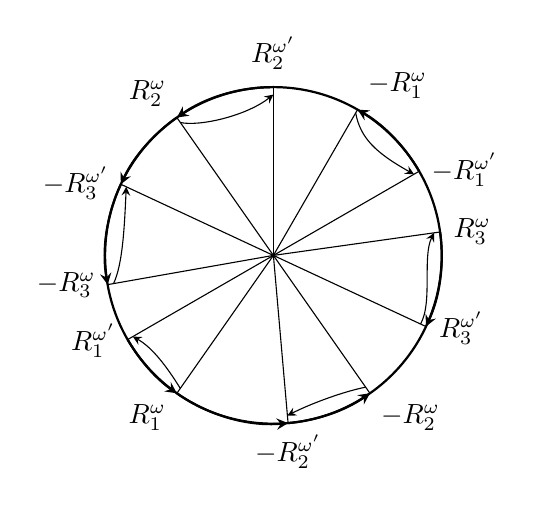
\begin{tikzpicture}[x=0.95cm,y=0.95cm,>=stealth]
\draw[thick] (0,0) circle (2.25);
\foreach \a in {90,125,60,30,8,-25,-55,-85,-125,-150,-170,155}{\draw[thin] (0,0)--(\a:2.25);}
\node[above] at (90:2.35) {$R_2^{\omega'}$};
\node[above left] at (125:2.27) {$R_2^\omega$};
\node[above right] at (60:2.27) {$-R_1^\omega$};
\node[right] at (30:2.29) {$-R_1^{\omega'}$};
\node[right] at (8:2.3) {$R_3^\omega$};
\node[right] at (-25:2.3) {$R_3^{\omega'}$};
\node[below right] at (-55:2.28) {$-R_2^\omega$};
\node[below] at (-85:2.28) {$-R_2^{\omega'}$};
\node[below left] at (-125:2.28) {$R_1^\omega$};
\node[left] at (-150:2.28) {$R_1^{\omega'}$};
\node[left] at (-170:2.28) {$-R_3^\omega$};
\node[left] at (155:2.28) {$-R_3^{\omega'}$};
\draw[->,thick] (90:2.25) arc (90:125:2.25);
\draw[->] (125:2.17) .. controls (-1.0,1.72) and (-0.37,1.86) .. (90:2.15);
\draw[->,thick] (125:2.25) arc (125:155:2.25);
\draw[->] (60:2.2) .. controls (1.16,1.57) and (1.37,1.37) .. (30:2.17);
\draw[->,thick] (30:2.25) arc (30:60:2.25);
\draw[->,thick] (8:2.25) arc (8:-25:2.25);
\draw[->] (-25:2.17) .. controls (2.13,-0.64) and (1.99,-0.01) .. (8:2.17);
\draw[->,thick] (-85:2.25) arc (-85:-55:2.25);
\draw[->] (-55:2.15) .. controls (0.89,-1.83) and (0.44,-2.01) .. (-85:2.15);
\draw[->,thick] (-125:2.25) arc (-125:-85:2.25);
\draw[->,thick] (-150:2.25) arc (-150:-125:2.25);
\draw[->] (-125:2.17) .. controls (-1.43,-1.48) and (-1.62,-1.23) .. (-150:2.17);
\draw[->,thick] (155:2.25) arc (155:190:2.25);
\draw[->] (-170:2.17) .. controls (-2.01,-0.11) and (-1.99,0.43) .. (155:2.17);
\end{tikzpicture}%
}

$P_i^{\omega,\zeta}$ prend $12$ valeurs distinctes

\unsure{pq|puis} six valeurs pour \deleted{$\unsure{P_i^\omega}$} $\zeta$ fixé (les $P_i^\omega$) et les six

\figure{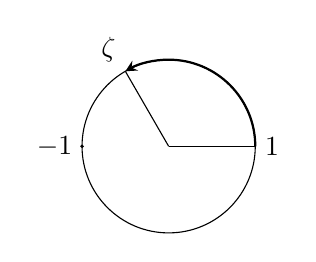
\begin{tikzpicture}[>=stealth]
\draw (0,0) circle (1.1);
\draw (0,0)--(1.1,0);\draw (0,0)--(120:1.1);
\draw[->,thick] (1.1,0) arc (0:120:1.1);
\fill (-1.1,0) circle (0.025);\node[left] at (-1.1,0) {$-1$};
\node[right] at (1.1,0) {$1$};\node[above left] at (120:1.1) {$\zeta$};
\end{tikzpicture}}

\[
Q_i^\omega=R_j-R_k\longmapsto R_j-\zeta R_k
=P_i^{\omega\deleted{\unsure{\zeta}}}=P_i^{\omega,\zeta}
\]
\[
P_i^{\omega,\zeta}=R_{\omega i}\deleted{\unsure{\zeta}}-\zeta R_{\omega^{\unsure{2|4}}i}
\qquad=-P_{\omega^2i}^{\omega,\zeta}
\]
\[
P_i^{\omega',\zeta'}=R_{\omega'i}-\zeta'R_{\omega i}
=R_k-\zeta^2R_j=-\zeta'P_i^{\omega,\zeta}
\]

\mspage{112}

\scanpage{114}
\mspage{1}

Carte $X$ (pas orientée)\inserted{\unsure{finie|fermée}}, $\mathcal R$ ens. des repères,
$S=\underset{\text{sommets}}{S_0}\amalg\underset{\text{arêtes}}{S_1}\amalg\underset{\text{faces}}{S_\infty}$
l'ens. de ces \unsure{facettes}, identifiées à \deleted{\unsure{aux}} leurs centres, donc si on désigne par $X$ aussi la \unsure{surface} topologique sous-jacente : $X$, on a
\[
 S=S_0\amalg S_1\amalg S_\infty\subset X.
\]

si $\varphi\in S$, on désigne par $R_\varphi$ le sommet associé. On identifie un $r=(s,a,f)\in\mathcal R$ à la région triangulaire correspondante (c'est un triangle de la subdivision barycentrique), de sommets $R_s,R_a,R_f$, d'indices respectifs $0,1,\infty$. On oriente ce triangle dans le sens $0,1,\infty$ (orientation du repère). Les régions ``adjacentes'' sont $\tau_0(r),\tau_1(r),\tau_\infty(r)$, opposées respectivement aux sommets de type $0,1,\infty$ de $r$. Notons
\[
 (1)\quad
 \left\{\begin{aligned}
 \tau_1(\tau_0(r))&=\rho_\infty(r)\\
 \tau_0(\tau_1(r))&=\rho_\infty^{-1}(r)
 \end{aligned}\right.
 \qquad\text{(face conservée)}
\]
\unsure{déduits|différents} de $r$ par ``rotation'' d'un cran autour du sommet du type $\infty$ resp. $0$, dans le sens \deleted{indiqué} de l'orientation définie par $r$ resp. dans le sens opposé. On a de $\unsure{=}$

\figure{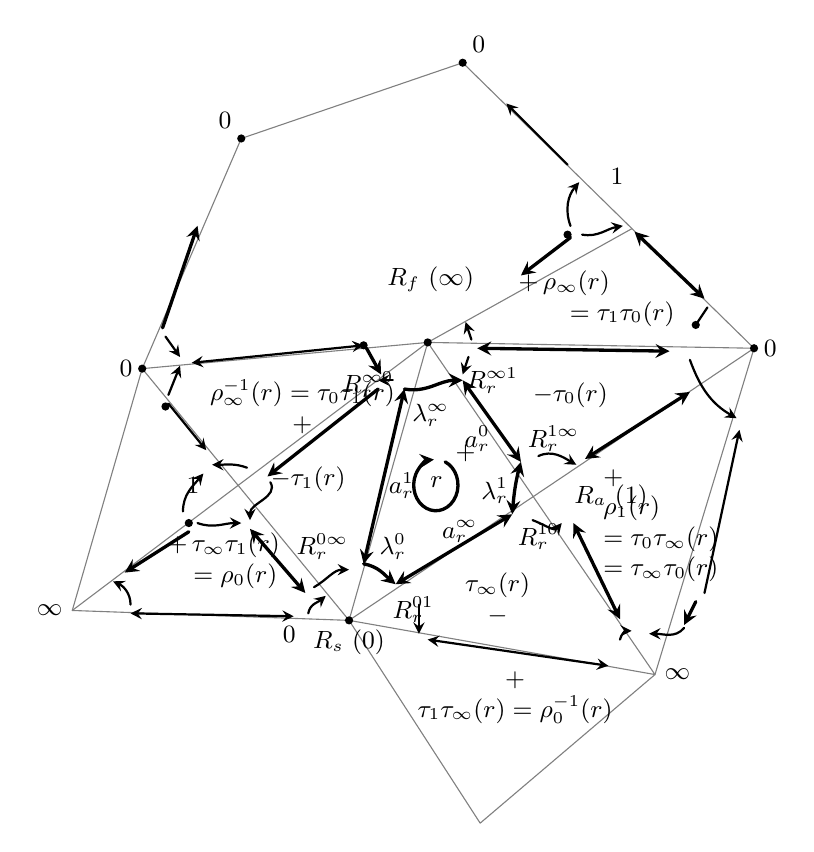
\begin{tikzpicture}[scale=.74,>=stealth,every node/.style={font=\small},line cap=round,line join=round]
\coordinate (T) at (7.5,-.6);
\coordinate (TL) at (3.7,-1.9);
\coordinate (L) at (2,-5.85);
\coordinate (LL) at (.8,-10);
\coordinate (F) at (6.9,-5.4);
\coordinate (S) at (5.55,-10.17);
\coordinate (A) at (9.5,-7.5);
\coordinate (TR) at (10.4,-3.45);
\coordinate (R) at (12.5,-5.5);
\coordinate (BR) at (10.8,-11.1);
\coordinate (B) at (7.8,-13.65);
\coordinate (AL) at (3.15,-7.5);
\draw[thin,gray] (TL)--(T)--(R)--(BR)--(B)--(S)--(LL)--(L)--cycle;
\draw[thin,gray] (L)--(S) (LL)--(F)--(R) (F)--(TR) (F)--(S) (F)--(BR) (S)--(R) (S)--(BR);
\draw[thin,gray] (L)--(F);
\foreach \p in {T,TL,L,F,S,R} \fill (\p) circle (2pt);
\node[above right] at (T) {$0$};
\node[above left] at (TL) {$0$};
\node[left] at (L) {$0$};
\node[left] at (LL) {$\infty$};
\node[right] at (R) {$0$};
\node[right] at (BR) {$\infty$};
\node[below] at (S) {$R_s\ (0)$};
\node[above] at (6.95,-4.7) {$R_f\ (\infty)$};
\node[right] at (9.25,-8.05) {$R_a\ (1)$};
\node[above] at (10.15,-2.85) {$1$};
\node[left] at (3.15,-7.85) {$1$};
\node[below left] at (4.8,-10.1) {$0$};
\draw[->,very thick] (2.35,-5.15)--(2.95,-3.4);
\draw[->,thick] (9.3,-2.35)--(8.25,-1.3);
\draw[<->,very thick] (10.45,-3.5)--(11.65,-4.65);
\draw[->,very thick] (9.35,-3.6)--(8.5,-4.25);
\draw[->,thick] (9.35,-3.4) to[out=110,in=230] (9.5,-2.65);
\draw[->,thick] (9.55,-3.55) to[out=-10,in=190] (10.25,-3.4);
\fill (9.3,-3.55) circle (2pt);
\fill (11.5,-5.1) circle (2pt);
\draw[thick] (11.7,-4.8)--(11.5,-5.1);
\draw[->,thick] (11.4,-5.7) to[out=-70,in=150] (12.2,-6.7);
\draw[->,thick] (11.65,-9.7)--(12.25,-6.9);
\draw[<->,very thick] (9.4,-8.5)--(10.2,-10.15);
\draw[->,thick] (10.2,-10.5) to[out=80,in=180] (10.4,-10.35);
\draw[->,thick] (11.3,-10.3) to[out=-130,in=0] (10.7,-10.4);
\draw[->,very thick] (11.5,-9.85)--(11.3,-10.25);
\draw[<->,thick] (6.9,-10.5)--(10,-10.95);
\draw[->,thick] (6.75,-9.9)--(6.75,-10.4);
\draw[<->,thick] (1.8,-10.05)--(4.6,-10.1);
\draw[->,thick] (1.8,-9.9) to[out=90,in=-25] (1.5,-9.5);
\draw[->,very thick] (2.8,-8.65)--(1.7,-9.35);
\fill (2.8,-8.5) circle (2pt);
\draw[->,thick] (2.7,-8.3) to[out=90,in=230] (3.05,-7.65);
\draw[->,thick] (2.95,-8.5) to[out=-20,in=180] (3.7,-8.5);
\draw[->,thick] (4.2,-7.8) to[out=-60,in=90] (3.85,-8.45);
\draw[->,thick] (3.8,-7.55) to[out=160,in=0] (3.2,-7.5);
\draw[<->,very thick] (3.85,-8.6)--(4.8,-9.7);
\draw[->,thick] (4.85,-10.05) to[out=80,in=-140] (5.15,-9.75);
\draw[->,thick] (4.95,-9.6) to[out=30,in=180] (5.55,-9.3);
\draw[->,thick] (2.45,-6.45)--(3.1,-7.25);
\fill (2.4,-6.5) circle (2pt);
\draw[->,thick] (2.45,-6.3)--(2.65,-5.8);
\draw[->,thick] (2.4,-5.3)--(2.65,-5.65);
\draw[<->,thick] (2.85,-5.75)--(5.8,-5.45);
\fill (5.8,-5.45) circle (2pt);
\draw[->,very thick] (5.85,-5.5)--(6.1,-5.95);
\draw[->,thick] (6.3,-6.05)--(6.05,-6.05);
\draw[->,very thick] (6.05,-6.2)--(4.15,-7.7);
\draw[<->,very thick] (7.75,-5.5)--(11.05,-5.55);
\draw[->,thick] (7.65,-5.35)--(7.55,-5.05);
\draw[->,thick] (7.6,-5.65)--(7.5,-5.95);
\draw[<->,very thick] (9.6,-7.4)--(11.4,-6.25);
\draw[->,thick] (8.8,-7.35) to[out=25,in=150] (9.45,-7.5);
\draw[->,thick] (8.7,-8.45) to[out=-20,in=230] (9.2,-8.5);
\coordinate (F0) at (6.5,-6.2);
\coordinate (F1) at (7.5,-6.05);
\coordinate (Ainf) at (8.5,-7.45);
\coordinate (A0) at (8.35,-8.35);
\coordinate (S1) at (6.35,-9.55);
\coordinate (Sinf) at (5.8,-9.2);
\draw[<->,very thick] (Sinf)--(F0);
\draw[->,very thick] (F0) to[out=-10,in=180] (F1);
\draw[<->,very thick] (F1)--(Ainf);
\draw[<->,very thick] (Ainf) to[out=-105,in=85] (A0);
\draw[<->,very thick] (A0)--(S1);
\draw[->,very thick] (Sinf) to[out=-10,in=140] (S1);
\draw[->,very thick] (7.2,-7.45) arc[start angle=65,end angle=-265,x radius=.38,y radius=.44];
\node at (7.05,-7.8) {$r$};
\node at (7.55,-7.3) {$+$};
\node at (6.45,-7.85) {$a_r^1$};
\node at (7.75,-7.05) {$a_r^0$};
\node at (7.45,-8.65) {$a_r^\infty$};
\node at (6.95,-6.65) {$\lambda_r^\infty$};
\node at (8.05,-7.95) {$\lambda_r^1$};
\node at (6.3,-8.9) {$\lambda_r^0$};
\node[anchor=east] at (6.48,-6.12) {$R_r^{\infty 0}$};
\node[anchor=west] at (7.4,-6.05) {$R_r^{\infty 1}$};
\node[anchor=west] at (8.45,-7.05) {$R_r^{1\infty}$};
\node[anchor=north] at (8.8,-8.35) {$R_r^{10}$};
\node[anchor=east] at (5.7,-8.9) {$R_r^{0\infty}$};
\node[anchor=north] at (6.65,-9.6) {$R_r^{01}$};
\node at (4.85,-7.75) {$-\tau_1(r)$};
\node at (9.35,-6.3) {$-\tau_0(r)$};
\node[align=center] at (8.1,-9.8) {$\tau_\infty(r)$\\$-$};
\node[align=center] at (4.75,-6.5) {$\rho_\infty^{-1}(r)=\tau_0\tau_1(r)$\\$+$};
\node[align=left] at (9.8,-4.65) {$+\,\rho_\infty(r)$\\$\qquad=\tau_1\tau_0(r)$};
\node[align=left] at (3.4,-9.15) {$+\,\tau_\infty\tau_1(r)$\\$\quad=\rho_0(r)$};
\node[align=center] at (8.4,-11.5) {$+$\\$\tau_1\tau_\infty(r)=\rho_0^{-1}(r)$};
\node[align=left] at (10.9,-8.55) {$+$\\$\unsure{\rho_1(r)}$\\$=\tau_0\tau_\infty(r)$\\$=\tau_\infty\tau_0(r)$};
\end{tikzpicture}}

\[
 (2)\quad
 \left\{\begin{aligned}
 \tau_\infty\tau_1(r)&=\rho_0(r)\\
 \tau_1\tau_\infty(r)&=\rho_0^{-1}(r)
 \end{aligned}\right.
 \qquad\text{(sommet conservé)}
\]
où $\rho_0$ est la rotation \inserted{d'un cran} autour du sommet de type $0$, dans le sens indiqué par l'orientation choisie pour $r$. Enfin
\[
 (3)\qquad\tau_0\tau_\infty(r)=\tau_\infty\tau_0(r)\overset{\mathrm{def}}=\rho_1(r),
\]

[ Pour mémoire, les relations dans le groupe cartographique
\[
 (4)\qquad\tau_0^2=\tau_1^2=\tau_\infty^2=(\tau_0\tau_\infty)^2=1
\]
\[
 (5)\quad
 \left\{\begin{aligned}
 \rho_\infty&=\tau_1\tau_0\\
 \rho_0&=\tau_\infty\tau_1\\
 \rho_1&=\tau_0\tau_\infty
 \end{aligned}\right.
 \qquad\rho_\infty\rho_1\rho_0\deleted{\unsure{\rho_\infty}}=1
 \qquad\text{]}
\]
\mspage{113}

\scanpage{115}
\mspage{2}

On introduit des sommets
\[
(6)\qquad R_r^{i,j}\qquad r\in\mathcal{R},\quad (i,j)\in\operatorname{\unsure{Rep|Coup}}\{0,1,\infty\}\quad\text{i.e. }i,j\in\{0,1,\infty\},\ i\ne j
\]
comme indiqués, \uline{satisfaisant} aux seules relations
\[
(7)\qquad \boxed{R_r^{ij}=R_{\unsure{\sigma_k(r)|\tau_k(r)}}^{i,j}}\quad k\notin\{i,j\}.
\]
On dit que $R_r^{ij}$ est ``proche'' du $R_r^i$ \inserted{sommet de $r$} ($=R_s,R_{\unsure{o|a}},R_f$ suivant que $i=0,1,\infty$), il se trouve sur le côté \deleted{\unsure{du plus proche}} \inserted{qui joint celui-ci} \deleted{\unsure{sommet opposé}} au sommet de type $j$.

On introduit des arcs
\[
(8)\qquad \lambda_r^i:R_r^{i,i+1}\longrightarrow R_r^{i,i+2}\qquad r\in\mathcal{R},\ i\in\{0,1,\infty\}
\]
\[
(9)\qquad a_r^i:R_r^{\deleted{\unsure{i+2}}\unsure{i},i+1}\longrightarrow R_r^{i+1,i+2}\qquad r\in\mathcal{R},\ i\in\{0,1,\infty\}
\]
\margin{\uline{NB} On écrit pour simplifier $i+1$ au lieu du résultat de la permutation circulaire $(0,1,\infty)\longmapsto(1,\infty,0)$, i.e. on identifie $\{0,1,\infty\}$ à $\mathbb{Z}/3\mathbb{Z}\ldots$}
\deleted{qui} \inserted{les $a_r^i$} entourent le disque repéré $r$ en formant un contour fermé dans le sens \deleted{opposé} \inserted{de} l'orientation de $r$ --- \deleted{par contre les} \inserted{\unsure{de = disques}} $\lambda_r^i$ \deleted{\unsure{sont}} \deleted{\unsure{une}} portions d'arc tournant autour des sommets de $r$ de type $i$ dans le sens correspondant à l'orientation de $r$. (Cela \deleted{\unsure{nous}} semble préférable à la convention de notation inverse). On a les seules \deleted{identités} relations
\[
(10)\qquad \boxed{a_r^i=a_{\tau_i(r)}^i}.
\]
\margin{\uline{NB} On désigne par les \deleted{\unsure{ces}} lettres minuscules les flèches obtenues après bouchage de certains trous.}
\margin{(\uline{NB} \unsure{si|i.e.} on bouche les disques $\overline{R}_r^i$, \unsure{où|et} $\lambda_r^i$ devient $=1$)}

\deleted{On désigne}
\uline{NB} On \unsure{suppose} que $X$ \unsure{est} \unsure{condition de trans-} \unsure{réalisée} par sa réalisation conforme canonique, qui est une surface $\mathbb{C}$ analytique réelle donc $C^\infty$, dont on peut considérer son éclaté en les $R_q$ $(q\in S)$ et le découpage de l'éclaté, qui est une surface à bord analytique réelle (mais pas conforme) dont l'intérieur coïncide avec $X\setminus S$, on le note

\mspage{114}

\scanpage{116}

$\widetilde{X}^{\substack{*\\*}*}$ ; (les trois $*$ signifient qu'on a enlevé \inserted{tous} les points de type $0,1,\infty$, disposés comme suit $\substack{\infty\\0}1$, on définirait de même $\widetilde{X}^{\substack{*\\\cdot}*}$, $\widetilde{X}^{\substack{\cdot\\*}*}$, $\widetilde{X}^{\substack{*\\*}\cdot}$, etc. \deleted{\unsure{Donc}} L'intérieur de cette surface à bord, savoir $X\setminus S=X\setminus\{R_q\mid q\in S\}$, est notée $X^{\substack{*\\*}*}$, on définit de \unsure{=} $X^{\substack{*\\\cdot}*}$ etc. Les points $R_r^{ij}$ et les chemins précédents seront regardés, le plus commodément, comme points et chemins (parfaitement canoniques, pas seulement des classes d'homotopie !) dans $\widetilde{X}^{\substack{*\\*}*}$. On notera que les $R_q$ $(q\in S)$ ne \uline{sont pas} dans $\widetilde{X}^{\substack{*\\*}*}$ --- mais dans l'application $C^\infty$ ($\unsure{\ne|\text{non}}$ analytique réelle) canonique
\diagram{
\begin{tikzcd}[ampersand replacement=\&]
\widetilde{X}^{\substack{*\\*}*} \arrow[r] \& X
\end{tikzcd}
\quad $(11)$
}
Le point $R_r^{ij}$ va sur $R_r^i=R_q$, où $q$ est le \uuline{sommet} de type $i$ de $r$.

On a, dans $\Pi_1 X^{\substack{*\\*}*}$, la relation
\[
(12)\qquad
\boxed{
\underbrace{(\lambda_r^0)^{-1}a_r^1}_{\underset{=}{\text{déf}}\ b_r^\infty}
\underbrace{{\lambda_r^\infty}^{-1}a_r^0}_{b_r^1}
\underbrace{(\lambda_r^1)^{-1}a_r^\infty}_{b_r^0}=1
}
\qquad\text{le tout en }R_r^{1\infty}
\]
\figure{
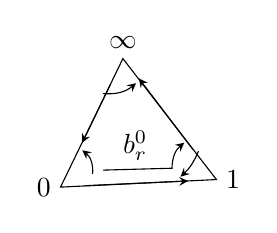
\begin{tikzpicture}[scale=1.2,>=stealth]
\coordinate (O) at (0,0);\coordinate (A) at (1.65,0.08);\coordinate (B) at (0.66,1.36);
\draw (O)--(A)--(B)--cycle;
\draw[->] (0.26,0.015)--(1.35,0.065);
\draw[->] (1.40,0.40)--(0.83,1.15);
\draw[->] (0.53,1.09)--(0.23,0.47);
\draw[->] (0.45,0.99) to[bend right=22] (0.80,1.10);
\draw[->] (0.34,0.14) to[bend right=28] (0.23,0.39);
\draw[->] (0.45,0.18)--(1.18,0.20) to[bend left=25] (1.31,0.47);
\draw[->] (1.46,0.38) to[bend left=12] (1.27,0.11);
\node[left] at (O) {$0$};\node[right] at (A) {$1$};\node[above] at (B) {$\infty$};
\node at (0.79,0.44) {$b_r^0$};
\end{tikzpicture}
}
Les sommets $R_r^{ij}$, les flèches $\lambda_r^i$ et $a_r^i$, et les relations $(10)$ $(12)$, forment une présentation du groupoïde $\Pi_1(\widetilde{X}^{\substack{*\\*}*},\{R_r^{ij}\})$.

\mspage{115}

\scanpage{117}
\mspage{3}

Les notations introduites sont telles qu'elles gardent un sens pour toute carte triangulaire ``polarisée'' de type $\{0,1,\infty\}$, sans que celle\deleted{\unsure{qui est la}} \inserted{-ci soit} nécessairement : la subdivision barycentrique d'une carte $X$, condition qui s'exprime par la \deleted{\unsure{condition}} \inserted{dernière} relation
\[
\deleted{\unsure{\tau_0}}\qquad (\tau_0\tau_\infty)^2=1\qquad\text{i.e.}\quad\rho_1^2=1
\]
dans $(4)$ (qu'on abandonne donc par la suite) et qui signifie aussi que les \deleted{points} \inserted{sommets} de type $1$ sont d'ordre réduit $2$ (d'ordre ordinaire $4$), ou encore que $\tau_0\tau_\infty(r)=\tau_\infty\tau_0(r)$ pour tout $r$. Dans le cas général, $\rho_1$ est donc une op. qui ne joue plus un rôle particulier p.r. à $\rho_0,\rho_\infty$ : c'est la rotation ``d'un cran'' de $r$ autour du sommet de type $1$, dans le \deleted{\unsure{demi-tour défini}} \inserted{sens défini} par l'orientation de $r$.

On introduit
\[
(13)\qquad\left\{
\begin{aligned}
\Lambda_r^i&=(\lambda_{\unsure{\tau_{i+1}r|\tau_{i+1}}}^i)^{-1}\lambda_r^i:R_r^{i,i+1}\mathrel{\unsure{-|\longrightarrow}} R_{\tau_{i+1}(r)}^{i,i+1}\\
\Lambda_r^{\prime i}&=\lambda_{\unsure{\sigma_{i-1}(r)|\tau_{i-1}(r)}}^i(\lambda_r^i)^{-1}:R_r^{i,i-1}\mathrel{\unsure{-|\longrightarrow}} R_{\tau_{i-1}(r)}^{\unsure{i-1|i,i-1}}
\end{aligned}\right.
\]
rotation d'un double ``cran'' autour du sommet de type $i$ de $r$, à partir du sommet proche de type $(i,i+1)$, \inserted{resp. $(i,i-1)$}, dans le sens de rotation donné par l'orientation de $r$. \inserted{resp. en sens opposé} On a les relations

\figure{
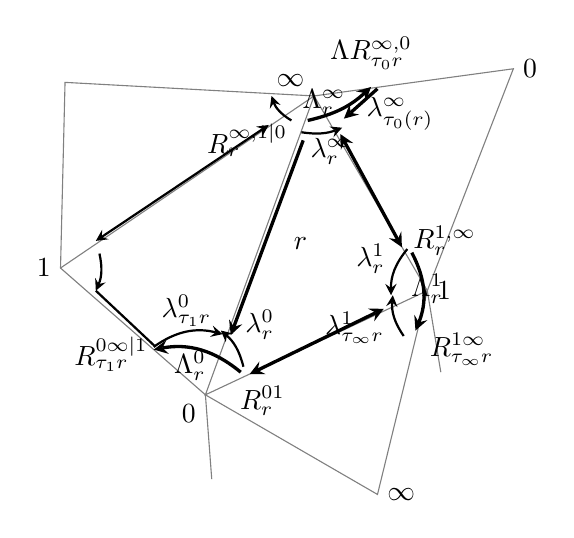
\begin{tikzpicture}[scale=1.15,>=stealth]
\coordinate (A) at (1.75,0.95);\coordinate (B) at (4.2,2.1);\coordinate (C) at (2.95,4.25);
\coordinate (D) at (0.15,2.35);\coordinate (E) at (5.15,4.55);\coordinate (F) at (3.65,-0.15);\coordinate (G) at (0.2,4.4);
\draw[gray] (G)--(C)--(E)--(B)--(F)--(A)--(D)--cycle;
\draw[gray] (A)--(B)--(C)--cycle (D)--(C) (A)--(1.82,0.02) (B)--(4.35,1.2);
\draw[very thick,->] (2.83,3.76)--(2.03,1.61);
\draw[very thick,<->] (2.24,1.18)--(3.72,1.9);
\draw[very thick,<->] (3.92,2.58)--(3.24,3.83);
\draw[thick,<->] (0.54,2.65)--(2.45,3.93);
\draw[thick,->] (0.58,2.51) to[bend left=18] (0.54,2.10);
\draw[thick] (0.54,2.10)--(1.20,1.48);
\draw[thick,->] (2.17,1.26) to[bend right=18] (1.92,1.66);
\draw[thick,->] (1.18,1.48) to[bend left=25] (1.94,1.62);
\draw[very thick,->] (2.14,1.20) to[bend right=25] (1.18,1.45);
\draw[thick,->] (3.98,2.56) to[bend right=20] (3.80,2.05);
\draw[thick,->] (3.94,1.60) to[bend left=20] (3.82,2.05);
\draw[very thick,->] (4.03,2.52) to[bend left=25] (4.07,1.66);
\draw[thick,->] (2.81,3.85) to[bend right=15] (3.26,3.90);
\draw[thick,->] (2.70,3.98) to[bend left=20] (2.48,4.25);
\draw[very thick,->] (2.88,3.98) to[bend right=15] (3.58,4.35);
\draw[very thick,->] (3.65,4.33)--(3.28,4.00);
\node[below left] at (A) {$0$};\node[right] at (B) {$1$};\node[above left] at (C) {$\infty$};
\node[left] at (D) {$1$};\node[right] at (E) {$0$};\node[right] at (F) {$\infty$};\node at (2.8,2.62) {$r$};
\node[below] at (2.38,1.15) {$R_r^{01}$};
\node[left] at (1.22,1.40) {$R_{\tau_1r}^{0\unsure{\infty|1}}$};
\node at (1.54,1.88) {$\lambda_{\tau_1r}^0$};\node at (1.58,1.27) {$\Lambda_r^0$};\node at (2.35,1.72) {$\lambda_r^0$};
\node[right] at (3.94,2.65) {$R_r^{1,\infty}$};\node[right] at (4.12,1.45) {$R_{\tau_\infty r}^{1\infty}$};
\node[left] at (3.84,2.45) {$\lambda_r^1$};\node[left] at (3.83,1.69) {$\lambda_{\tau_\infty r}^1$};\node at (4.20,2.12) {$\Lambda_r^1$};
\node[left] at (2.76,3.76) {$R_r^{\infty,\unsure{1|0}}$};\node[above] at (3.58,4.44) {$\deleted{\unsure{\Lambda}}R_{\tau_0r}^{\infty,0}$};
\node at (3.13,3.64) {$\lambda_r^\infty$};\node at (3.90,4.05) {$\lambda_{\tau_0(r)}^\infty$};\node at (3.06,4.18) {$\Lambda_r^\infty$};
\end{tikzpicture}
}
\[
(14)\qquad \boxed{\Lambda_r^i\Lambda_{\tau_{i+1}(r)}^i=1}\qquad
\boxed{\Lambda_r^{\prime i}\Lambda_{\tau_{i-1}(r)}^{\prime i}=1}.
\]

\mspage{116}

\scanpage{118}
\mspage{117}
\mspage{4}
\deleted{Soit} $i$

\deleted{L'introduction des $\Lambda_r^i$}

Fixons nous un indice dans $\{0,1,\infty\}$, disons $1$ (en pensant au cas où la triangulation est barycentrique, donc \inserted{où} $1$ joue un rôle particulier !). Nous pouvons éliminer les sommets $R_r^{ij}$ qui se trouvent sur des côtés de $r$ qui sont de type $1$, i.e. pour lesquels $i,j\ne1$, et l'arc $a_r^1$ qui les joint, en gardant les sommets
\[
(14)\qquad\left\{R_r^{i,j}\quad\left\{\begin{array}{l}
r\in\mathcal{R}\\
i\text{ ou }j\text{ est égal à }1\quad\text{i.e.}\quad\{i,j\}\ne\{0,\infty\}
\end{array}\right.\right.
\]
et les arcs
\[
(15)\qquad\left\{\begin{array}{ll}
\lambda_r^1&r\in\mathcal{R}\\
\Lambda_r^0,\Lambda_r^{\prime\infty}&r\in\mathcal{R},\quad\deleted{\unsure{i\in\{0,\infty\}}}\\
a_r^i&r\in\mathcal{R},\quad i\in\{0,\infty\}
\end{array}\right.
\]
\margin{$\Lambda_r^0\Lambda_{\tau_1r}^0=$}
avec comme relations les relations $(14)$ de redondance \inserted{pour $i=0$ et $i=\infty$} \deleted{\unsure{et les relations du type} $\unsure{\Lambda_r^0}=\unsure{1}$}
\deleted{
\[
\boxed{
\Lambda_{\tau_1r}^{\unsure{\infty|\prime\infty}}
\underbrace{(a_{\tau_1r}^0(\lambda_{\tau_1r}^1)^{-1}a_{\tau_1r}^\infty)^{-1}}_{\beta_{\tau_1r}^{1\,-1}}
\Lambda_r^0\underbrace{a_r^\infty\lambda_r^1a_r^0}_{\unsure{\beta_r^1}}=1
}\qquad(16)
\]
pour $r\in\mathcal{R}$ (lacets en $R_r^{01}$)

\uline{NB} Cette relation est équivalente à la relation \deleted{\unsure{inverse}} \inserted{où $r$ est remplacé} par $\unsure{\sigma_1r|\tau_1r}$
}

\margin{pavage par des carrés ? (dont les sommets \unsure{qui ne sont} pas de type $1$, sont ``arrondis'', de façon à faire des hexagones \unsure{évitant} les trous}
\figure{
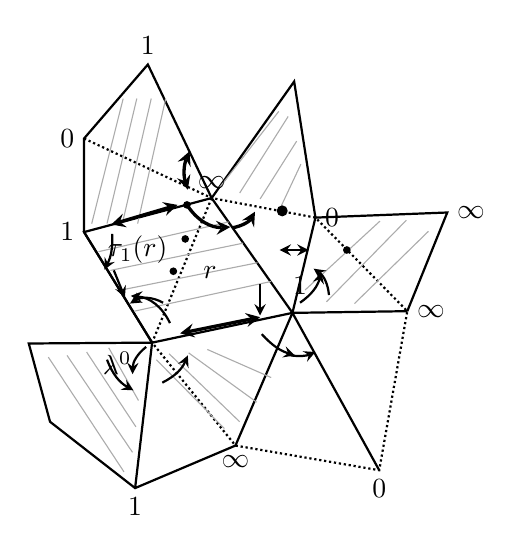
\begin{tikzpicture}[scale=1.08,>=stealth]
\coordinate (A) at (1.25,1.85);\coordinate (B) at (2.90,2.20);\coordinate (C) at (1.95,3.55);
\coordinate (D) at (0.45,3.15);\coordinate (E) at (0.45,4.25);\coordinate (F) at (1.20,5.12);
\coordinate (G) at (2.92,4.92);\coordinate (H) at (3.17,3.32);\coordinate (I) at (4.72,3.38);
\coordinate (J) at (4.25,2.22);\coordinate (K) at (3.92,0.35);\coordinate (L) at (2.23,0.64);
\coordinate (M) at (1.05,0.14);\coordinate (N) at (0.05,0.92);\coordinate (O) at (-0.20,1.84);
\draw[thick] (D)--(E)--(F)--(C) (C)--(G)--(H) (H)--(I)--(J) (B)--(J);
\draw[thick] (B)--(K) (B)--(L)--(M)--(N)--(O)--(A) (A)--(M) (A)--(D);
\draw[densely dotted,thick] (E)--(C)--(H)--(J)--(K)--(L)--(A)--(C);
\draw[thick] (D)--(C)--(B)--(A)--cycle (B)--(H);
\foreach \p/\q in {0.54/0.91,0.72/1.07,0.90/1.24,1.08/1.41}{\draw[gray!65] (\p,3.25)--(\q,4.72);}
\draw[gray!65] (2.04,3.67)--(2.74,4.57) (2.28,3.61)--(2.85,4.51) (2.52,3.54)--(2.95,4.22) (2.77,3.46)--(3.00,3.95);
\draw[gray!65] (3.05,2.47)--(3.93,3.28) (3.30,2.33)--(4.24,3.29) (3.63,2.31)--(4.50,3.16);
\draw[gray!65] (0.62,2.92)--(2.15,3.27) (0.76,2.70)--(2.32,3.02) (0.89,2.47)--(2.49,2.79) (1.04,2.22)--(2.65,2.57);
\draw[gray!65] (1.30,1.65)--(2.10,0.84) (1.45,1.72)--(2.28,0.92) (1.68,1.73)--(2.48,1.15) (1.90,1.77)--(2.65,1.44);
\draw[gray!65] (0.03,1.68)--(0.92,0.33) (0.25,1.70)--(1.02,0.56) (0.48,1.74)--(1.06,0.86) (0.74,1.79)--(1.09,1.17);
\fill (2.78,3.40) circle (0.065);\fill (1.66,3.47) circle (0.045);\fill (1.64,3.07) circle (0.045);\fill (1.50,2.69) circle (0.045);\fill (3.54,2.94) circle (0.045);
\draw[very thick,<->] (0.77,3.24)--(1.55,3.47);
\draw[very thick,<->] (1.67,3.65) to[bend left=20] (1.69,4.10);
\draw[very thick,->] (1.66,3.47) to[bend right=30] (2.17,3.21);
\draw[very thick,->] (2.19,3.20) to[bend right=25] (2.46,3.39);
\draw[thick,->] (0.78,3.13) to[bend left=15] (0.69,2.71);
\draw[thick,->] (0.80,2.70)--(0.93,2.38);
\draw[thick,->] (1.46,2.08) to[bend right=30] (1.00,2.40);
\draw[thick,->] (1.38,2.32) to[bend right=30] (0.99,2.31);
\draw[very thick,<->] (1.58,1.96)--(2.52,2.15);
\draw[thick,->] (2.52,2.54)--(2.52,2.17);
\draw[thick,<->] (2.75,2.94)--(3.09,2.94);
\draw[thick,->] (2.99,2.32) to[bend right=20] (3.24,2.68);
\draw[thick,->] (3.33,2.41) to[bend right=25] (3.15,2.72);
\draw[thick,->] (2.54,1.95) to[bend right=15] (2.93,1.70);
\draw[thick,->] (2.88,1.70) to[bend right=15] (3.17,1.74);
\draw[thick,->] (1.18,1.80) to[bend right=25] (1.02,1.48);
\draw[thick,->] (1.37,1.38) to[bend right=20] (1.67,1.70);
\draw[thick,->] (0.72,1.65) to[bend right=20] (1.03,1.29);
\node[above] at (F) {$1$};\node[left] at (E) {$0$};\node[left] at (D) {$1$};\node[above] at (C) {$\infty$};
\node[right] at (H) {$0$};\node[right] at (I) {$\infty$};\node[right] at (J) {$\unsure{\infty}$};\node[below] at (K) {$0$};
\node[below] at (L) {$\infty$};\node[below] at (M) {$1$};\node at (2.99,2.52) {$1$};
\node at (1.93,2.67) {$r$};\node at (1.08,2.94) {$\tau_1(r)$};\node at (0.84,1.61) {$\lambda^0$};
\end{tikzpicture}
}
\[
(16)\qquad\boxed{
\Lambda_{\tau_1(r)}^{\prime\infty}
\underbrace{(a_{\tau_1r}^0(\lambda_{\tau_1r}^1)^{-1}a_{\tau_1r}^\infty)^{\unsure{+|-1}}}_{\beta_{\tau_1(r)}^1\,\deleted{\unsure{-1}}}
\Lambda_r^0
\underbrace{((a_r^\infty)^{-1}\lambda_r^1(a_r^0)^{-1})}_{\beta_r^{1\,-1}}
=1
}
\]
\margin{relation stable par passage de $r$ à $\tau_1(r)$, donc il suffit de la poser pour $r\in\mathcal{R}^+$ (si $X$ orientable)}
\figure{
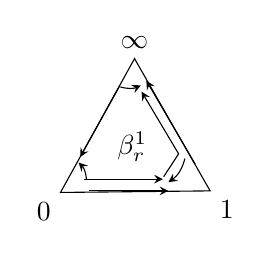
\begin{tikzpicture}[scale=1.0,>=stealth]
\coordinate (A) at (0,0);\coordinate (B) at (1.9,0.02);\coordinate (C) at (0.94,1.7);
\draw (A)--(B)--(C)--cycle;
\draw[->] (0.75,1.35)--(0.25,0.45);\draw[->] (0.36,0.02)--(1.37,0.02);\draw[->] (1.71,0.36)--(1.09,1.42);
\draw[->] (0.30,0.17)--(1.30,0.17);\draw[->] (1.31,0.20)--(1.50,0.49)--(1.03,1.28);
\draw[->] (0.76,1.34) to[bend right=20] (1.02,1.36);\draw[->] (0.33,0.16) to[bend right=20] (0.23,0.38);
\draw[->] (1.58,0.43) to[bend left=20] (1.37,0.13);
\node[below left] at (A) {$0$};\node[below right] at (B) {$1$};\node[above] at (C) {$\infty$};\node at (0.91,0.58) {$\beta_r^1$};
\end{tikzpicture}
}

\scanpage{119}

\figure{
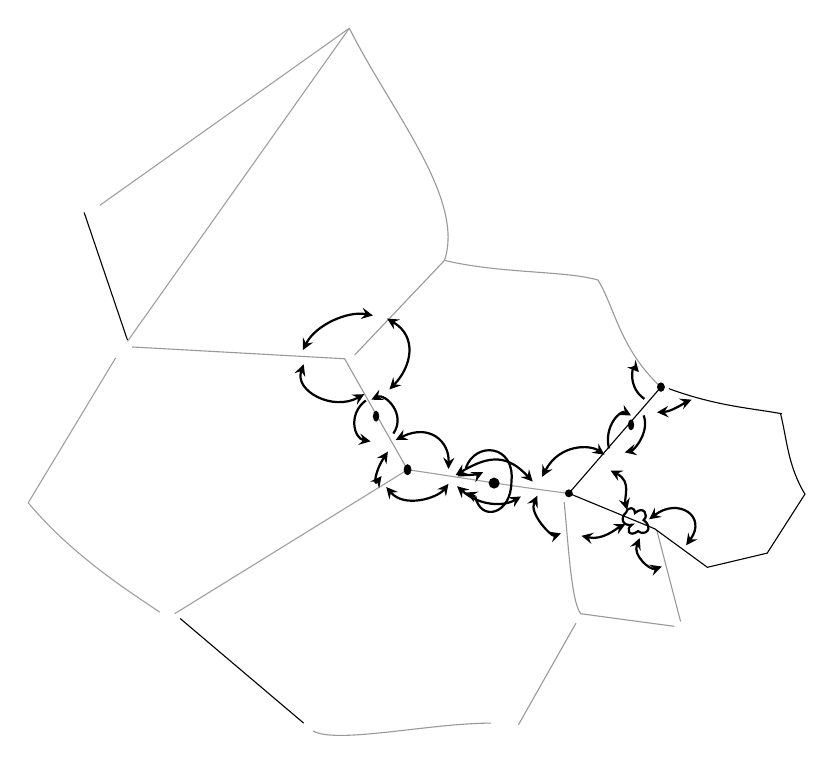
\begin{tikzpicture}[x=0.01cm,y=-0.01cm,>=stealth]
\draw[gray!75] (731,1307)--(1048,1082);
\draw[gray!75] (766,1480)--(1048,1082);
\draw (711,1316)--(766,1478);
\draw[gray!80] (1048,1082)..controls(1102,1189)and(1195,1298)..(1169,1377);
\draw[gray!80] (1169,1377)--(1055,1497);
\draw[gray!80] (772,1487)--(1042,1502)--(1122,1643);
\draw[gray!80] (1169,1377)..controls(1240,1394)and(1324,1390)..(1364,1402)..controls(1385,1436)and(1392,1490)..(1444,1538);
\draw[gray!75] (751,1501)--(640,1685)..controls(699,1756)and(780,1805)..(807,1824);
\draw[gray!75] (826,1826)--(1122,1643)..controls(1185,1652)and(1260,1665)..(1327,1673);
\draw (833,1832)--(990,1965);
\draw[gray!80] (1002,1975)..controls(1032,1992)and(1150,1965)..(1228,1965);
\draw[gray!80] (1263,1967)--(1336,1838);
\draw[gray!80] (1321,1684)..controls(1326,1734)and(1330,1811)..(1342,1826)--(1461,1842);
\draw[gray!80] (1439,1721)--(1469,1836);
\draw (1327,1673)--(1444,1538);
\draw (1327,1673)--(1436,1718)--(1503,1767)--(1579,1749)--(1627,1674)..controls(1605,1638)and(1604,1603)..(1596,1572);
\draw (1454,1540)..controls(1517,1563)and(1562,1565)..(1598,1572);
\fill (1082,1575) ellipse (4 and 7);\fill (1122,1643) ellipse (5 and 7);\fill (1232,1660) ellipse (7 and 7);
\fill (1327,1673) circle (5);\fill (1406,1586) ellipse (4 and 7);\fill (1444,1538) ellipse (5 and 6);
\draw[thick,<->] (989,1491)..controls(1005,1459)and(1046,1441)..(1078,1447);
\draw[thick,<->] (990,1509)..controls(978,1543)and(1027,1569)..(1067,1547);
\draw[thick,<->] (1096,1451)..controls(1135,1474)and(1127,1512)..(1099,1541);
\draw[thick,->] (1069,1555)..controls(1046,1572)and(1054,1603)..(1075,1607);
\draw[thick,->] (1104,1597)..controls(1121,1572)and(1093,1546)..(1076,1554);
\draw[thick,<->] (1097,1620)..controls(1080,1646)and(1079,1664)..(1089,1651);
\draw[thick,<->] (1107,1605)..controls(1150,1584)and(1175,1607)..(1174,1642);
\draw[thick,<->] (1095,1665)..controls(1118,1692)and(1160,1679)..(1174,1661);
\draw[thick,<->] (1183,1650)..controls(1228,1623)and(1250,1625)..(1281,1658);
\draw[thick,<->] (1185,1664)..controls(1213,1689)and(1244,1690)..(1266,1677);
\draw[thick,->] (1186,1650)..controls(1212,1650)and(1216,1647)..(1218,1646);
\draw[thick] (1196,1641)..controls(1208,1606)and(1259,1611)..(1254,1658)..controls(1254,1700)and(1215,1710)..(1208,1677);
\draw[thick,->] (1208,1677)--(1196,1672);
\draw[thick,<->] (1293,1652)..controls(1315,1610)and(1354,1611)..(1372,1624);
\draw[thick,<->] (1287,1676)..controls(1276,1699)and(1305,1728)..(1317,1724);
\draw[thick,<->] (1343,1727)..controls(1370,1733)and(1387,1718)..(1399,1712);
\draw[thick,<->] (1380,1644)..controls(1407,1658)and(1397,1678)..(1401,1694);
\draw[thick,->] (1378,1616)..controls(1371,1587)and(1393,1567)..(1406,1574);
\draw[thick,->] (1422,1574)..controls(1430,1595)and(1410,1618)..(1398,1621);
\draw[thick,->] (1423,1553)..controls(1401,1538)and(1408,1510)..(1416,1519);
\draw[thick,<->] (1439,1570)..controls(1458,1569)and(1478,1556)..(1483,1554);
\draw[thick] (1400,1697)..controls(1402,1689)and(1412,1691)..(1411,1698)..controls(1422,1688)and(1429,1701)..(1422,1707)..controls(1436,1718)and(1423,1728)..(1415,1721)..controls(1403,1730)and(1399,1718)..(1407,1713)..controls(1396,1715)and(1391,1705)..(1400,1697);
\draw[thick,<->] (1429,1706)..controls(1466,1678)and(1503,1702)..(1476,1739);
\draw[thick,<->] (1417,1730)..controls(1408,1752)and(1430,1771)..(1445,1766);
\end{tikzpicture}
}

Cas \uline{$\overline{\mathrm{IV}}$}

\mspage{118}

\scanpage{120}
\mspage{5}

On a donc trouvé $4=1+3$ présentations du groupoïde fondamental $\Pi_1(\widetilde{X}^{\substack{*\\*}*},S)$, suivant qu'on utilise tous les chemins $(8)$, $(9)$, ou qu'on élimine les chemins $a_r^i$ \inserted{($i$ fixé, dans l'exemple $i=1$)} et les sommets qui se trouvent dessus. Je vais maintenant examiner le cas où on élimine \unsure{=} deux côtés du triangle fondamental i.e. où on ne garde les $a_r^i$ que d'un seul type --- disons les $a_r^\infty$ --- ce qui conduit aussi à éliminer tous les sommets proches des $R_q$ \inserted{($q\in S$)} de type \deleted{infini} \inserted{$\infty$ et ceux qui leur sont reliés}, \deleted{\unsure{enfin}, des centres des faces} \inserted{etc.} --- i.e. \deleted{les $R_r^i$} à ne garder que les $R_r^{ij}$ avec \deleted{\unsure{pour}} \inserted{$(i,j)\in\{0,1\}$} \deleted{$\unsure{i,j\ne\infty}$, \unsure{les côtés ne passent pas par $\infty$})} :
\[
(17)\qquad R_r^{i,j}\quad\left\{\begin{array}{l}
r\in\mathcal{R}\\
\{i,j\}=\{0,1\}
\end{array}\right.
\]
\margin{$\left\{\begin{aligned}
R_r^{0,1}&=R_{\unsure{\tau_\infty r|\sigma_\infty r}}^{0,1}\\
R_r^{1,0}&=\unsure{Q|R}_{\tau_\infty(r)}
\end{aligned}\right.$ pour mémoire

relations de redondance}
\[
(18)\qquad\left\{\begin{aligned}
a_r^\infty &: R_r^{01}\deleted{\unsure{\to R}}\longrightarrow R_r^{1,0} \qquad(\forall r\in\mathcal{R})\\
\Lambda_r^0,\deleted{\Lambda_r^{\prime1}} &:R_r^{01}\longrightarrow R_{\tau_1r}^{01},\\
\Lambda_r^{\prime1} &:R_r^{10}\longrightarrow R_{\tau_0r}^{1,0},
\end{aligned}\right.
\]
\inserted{avec} relations de redondance seulement
\[
(19)\qquad\boxed{\begin{aligned}
\Lambda_r^0\Lambda_{\tau_1(r)}^0&=1\\
\Lambda_r^{\prime1}\Lambda_{\tau_0(r)}^{\prime1}&=1
\end{aligned}}
\]
\figure{
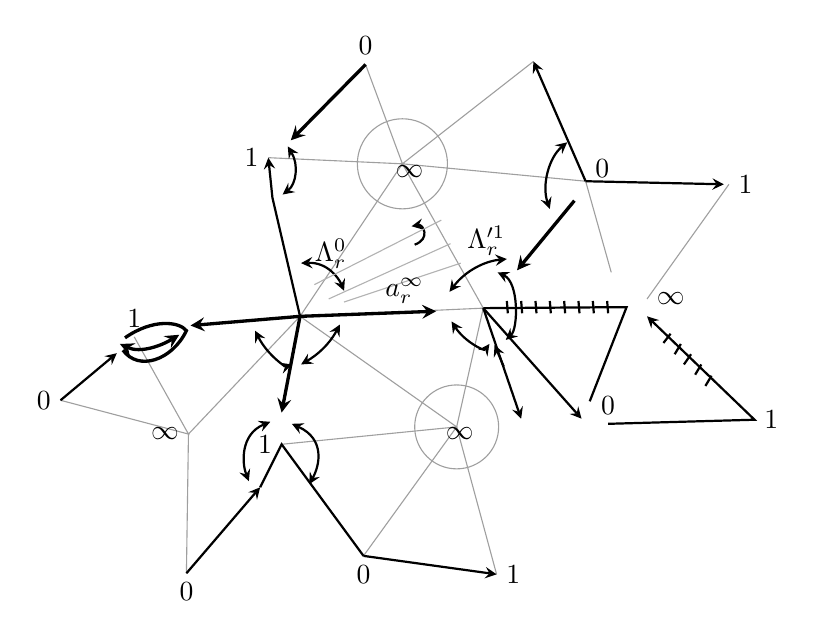
\begin{tikzpicture}[x=0.013cm,y=-0.013cm,>=stealth]
\draw[gray!75] (247,1588)--(378,1594)--(557,1611) (342,1497)--(378,1594)--(457,1735)--(278,1743)--(378,1594)--(506,1494);
\draw[gray!75] (116,1763)--(169,1858)--(44,1825) (169,1858)--(167,1994) (169,1858)--(278,1743)--(431,1851)--(260,1868);
\draw[gray!75] (457,1735)--(431,1851)--(340,1977) (431,1851)--(470,1995) (557,1611)--(582,1700) (617,1726)--(697,1614);
\draw[gray!75] (378,1594) circle (44);\draw[gray!75] (431,1851) circle (41);
\draw[very thick,->] (342,1497)--(269,1571);\draw[thick,->] (278,1743)--(251,1627)--(247,1588);
\draw[thick,<->] (266,1577)..controls(277,1595)and(274,1614)..(261,1624);
\draw[thick,->] (557,1611)--(506,1494);
\draw[thick,<->] (539,1573)..controls(521,1588)and(514,1615)..(522,1638);
\draw[thick,->] (557,1611)--(692,1614);
\draw[very thick,->] (546,1630)--(490,1698);
\draw[very thick,->] (278,1743)--(411,1738);
\draw[very thick,->] (278,1743)--(260,1837);
\draw[very thick,->] (278,1743)--(171,1752);
\draw[thick,<->] (279,1691)..controls(305,1690)and(316,1706)..(321,1718);
\draw[thick,<->] (424,1719)..controls(440,1698)and(459,1689)..(480,1687);
\draw[thick,<->] (234,1757)..controls(247,1782)and(264,1792)..(270,1790);
\draw[thick,<->] (279,1790)..controls(301,1777)and(310,1764)..(317,1751);
\draw[thick,->] (457,1735)--(494,1843);
\draw[thick,->] (457,1735)--(553,1843);
\draw[thick,->] (579,1848)--(722,1844)--(617,1743);
\draw[thick] (457,1735)--(597,1734)--(561,1826);
\foreach \x in {480,494,508,522,536,550,564,578}{\draw[thick] (\x,1728)--(\x+1,1740);}
\draw[thick] (640,1760)--(633,1769) (650,1770)--(644,1780) (660,1780)--(653,1790) (670,1790)--(664,1800) (680,1801)--(674,1811);
\draw[thick,<->] (471,1700)..controls(492,1710)and(491,1755)..(479,1766);
\draw[thick,<->] (426,1748)..controls(439,1768)and(458,1777)..(463,1770);
\draw[thick,->] (477,1792)--(468,1771);
\draw[thick,->] (167,1994)--(239,1910);\draw[thick] (239,1910)--(260,1868)--(340,1977);
\draw[thick,->] (340,1977)--(470,1995);
\draw[thick,<->] (249,1846)..controls(220,1858)and(221,1886)..(228,1904);
\draw[thick,<->] (270,1848)..controls(303,1863)and(297,1889)..(287,1907);
\draw[thick,->] (44,1825)--(99,1779);
\draw[very thick,<->] (102,1770)..controls(122,1779)and(142,1772)..(160,1761);
\draw[very thick] (107,1764)..controls(134,1745)and(160,1748)..(167,1757)..controls(153,1786)and(120,1797)..(105,1776);
\draw[thick,->] (390,1673)..controls(406,1667)and(398,1653)..(387,1655);
\draw[gray!60] (292,1712)--(416,1649) (306,1726)--(425,1672) (321,1729)--(435,1691);
\node[above] at (342,1497) {$0$};\node[left] at (247,1588) {$1$};\node at (385,1602) {$\infty$};
\node[right] at (557,1599) {$0$};\node[right] at (697,1614) {$\unsure{1}$};\node[right] at (617,1726) {$\infty$};
\node[above] at (579,1848) {$0$};\node[right] at (722,1844) {$1$};\node[right] at (470,1995) {$1$};
\node[below] at (340,1977) {$0$};\node[below] at (167,1994) {$0$};\node[left] at (260,1868) {$1$};
\node[left] at (169,1858) {$\infty$};\node[left] at (44,1825) {$0$};\node[above] at (116,1763) {$1$};\node at (434,1858) {$\infty$};
\node at (308,1682) {$\Lambda_r^0$};\node at (460,1669) {$\Lambda_r^{\prime1}$};\node at (380,1718) {$a_r^\infty$};
\end{tikzpicture}
}
\margin{pavage par des \inserted{faces} polygonales de centre des sommets de type $\infty$ --- les coins de ces polygones étant arrondis pour éviter les trous}

c'est donc directement exprimé comme un groupoïde libre. Cela fait trois autres présentations de $\Pi_1(X)$, mais sur des ens. de sommets différents, savoir $\Pi_1(\widetilde{X}^{\substack{*\\*}*},S-S_i)$, pour $i=\infty$ (cas explicité) ou $0$ ou $1$.

\mspage{119}

\scanpage{121}
\mspage{6}

Je vais donner \deleted{6} \inserted{trois} autres présentations, où on élimine non seulement les pts proches (disons) des \deleted{$\unsure{R_q}$} sommets de type $\infty$, \inserted{et les sommets qui leur sont liés \unsure{d'indice|d'arc} $\infty$} mais aussi ceux proches des sommets (disons) de type $1$, en gardant donc que les sommets \inserted{$R_r^{ij}$} de type $0$, i.e.
\[
(20)\qquad R_r^{0,1}\ \swarrow\qquad r\in\mathcal{R}
\]
\margin{$\boxed{R_r^{0,1}=R_{\unsure{\sigma_\infty r|\tau_\infty r}}^{01}}$

relations de redondance pour mémoire}
et on introduit les chemins
\[
(21)\qquad\left\{\begin{aligned}
A_r^{0,1}&\overset{\text{déf}}{=}(a_{\tau_0r}^\infty)^{-1}(\unsure{\Lambda_r^{\prime1}|\Lambda_r^1})^{-1}a_r^\infty:R_r^{01}\longrightarrow R_{\unsure{\sigma_0(r)|\tau_0(r)}}^{0,1}\qquad(r\in\mathcal{R})\\
\Lambda_r^0&:R_r^{0,1}\mathrel{\unsure{-|\longrightarrow}} R_{\unsure{\sigma_1r|\tau_1r}}^{01}\qquad(r\in\mathcal{R})
\end{aligned}\right.
\]
\margin{plus les chemins déjà connus}
on a les relations de redondance
\[
(22)\qquad\boxed{\left\{\begin{aligned}
\Lambda_r^0\Lambda_{\unsure{\tau_1(r)|\sigma_1(r)}}^0&=1&&r\in\mathcal{R}\\
A_r^{0,1}A_{\unsure{\sigma_0(r)|\tau_0(r)}}^{0,1}&=1&&r\in\mathcal{R}
\end{aligned}\right.}
\]
\figure{
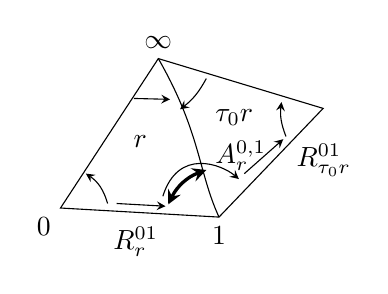
\begin{tikzpicture}[scale=1.15,>=stealth]
\coordinate (A) at (0,0);\coordinate (B) at (1.75,-0.10);\coordinate (C) at (1.08,1.65);\coordinate (D) at (2.90,1.10);
\draw (A)--(C)--(D)--(B)--cycle;
\draw (C)..controls(1.55,0.83)and(1.52,0.40)..(B);
\draw[->] (0.81,1.21)--(1.21,1.20);
\draw[->] (1.61,1.43) to[bend left=12] (1.32,1.09);
\draw[->] (0.52,0.05) to[bend right=20] (0.28,0.38);
\draw[->] (0.62,0.05)--(1.16,0.02);
\draw[very thick,<->] (1.19,0.04) to[bend left=22] (1.61,0.42);
\draw[->] (1.13,0.13)..controls(1.30,0.67)and(1.78,0.48)..(1.97,0.32);
\draw[->] (2.03,0.38)--(2.46,0.76);
\draw[->] (2.49,0.79) to[bend left=14] (2.44,1.17);
\node[below left] at (A) {$0$};\node[below] at (B) {$1$};\node[above] at (C) {$\infty$};
\node at (0.88,0.73) {$r$};\node at (1.92,1.00) {$\tau_0r$};\node at (1.99,0.58) {$A_r^{0,1}$};
\node[below] at (0.83,-0.10) {$R_r^{01}$};\node[right] at (2.50,0.53) {$R_{\tau_0r}^{01}$};
\end{tikzpicture}
}
et c'est tout : $\Pi_1(\widetilde{X}^{\substack{*\\*}*},\{R_r^{01}\}_{r\in\mathcal{R}})$ est \deleted{engendré} \inserted{présenté} par les sommets et flèches $(20)$ $(21)$, avec les seules relations de redondance $(20)$ $(22)$.

\uline{Bouchage \unsure{de|des} trous} Dans chacun des quatre cas envisagés, (en fait $10=1+3+3+3$ cas), le ``bouchage'' d'un trou $R_{\unsure{q|qs}}$ $(q\in S=S_0\amalg S_1\amalg S_\infty)$ se fait de façon essentiellement triviale. Dans chacun des quatre cas, il faut, en termes des flèches génératrices choisies, définir \unsure{\uline{les}|\deleted{les}}

\mspage{120}

\scanpage{122}
\mspage{7}

``lacet'' autour d'un tel $R_s$, puis exprimer que ce lacet est $\simeq1$.

\mspage{121}
